\documentclass[%
%draft,
11pt,%
twoside,%
titlepage,%
swissgerman,%
headsepline%
]{scrartcl}

\usepackage{lastpage}
\usepackage{amsthm}
\usepackage{amssymb}
\usepackage{geometry}
\usepackage{graphicx}
\usepackage[dvipsnames]{xcolor}
\usepackage[utf8]{inputenc}
\usepackage[swissgerman]{babel}
\usepackage{lscape}
\usepackage[framemethod=TikZ]{mdframed}
\usepackage[most]{tcolorbox}
\usepackage{enumerate}
\usepackage{units}
\usepackage{nicefrac}
\usepackage{pgf,tikz}
\usepackage{tikz-3dplot}
\usepackage{tkz-euclide}
\usetikzlibrary{arrows}
\usetikzlibrary{arrows.meta}
\usetikzlibrary{patterns}
\usetikzlibrary{positioning}
\usetikzlibrary{shadows}
\usetikzlibrary{quotes, angles}
\usepackage{colortbl}
\usepackage{hhline}
\usepackage{multirow}
\usepackage[extendedchars]{grffile}
\usepackage{caption}
\usepackage{multicol,calc}
\usepackage{blindtext}
\usepackage{pdfpages}
\usepackage{hyperref}
\usepackage{framed}

\usepackage{marginnote}
\usepackage{qrcode}
\qrset{height=9ex}

\usepackage{longtable}
\usepackage{listings}
\usepackage{wrapfig}

\usepackage{fontawesome} % Oder FontAwesome, falls du ein Augensymbol aus einer
\newcommand{\faEyeLightGray}{\textcolor{lightgray}{\faEye}} % Custom command for the gray eye icon
\newcommand{\faReturnGray}{\textcolor{gray}{\faMailReply}} % Custom command for the gray eye icon
\usepackage{pifont} % weitere Zeichen
\usepackage{eurosym}

% package für plots mit dem Befehl axes
\usepackage{pgfplots}
\pgfplotsset{compat=1.18}


% Command, um Tabellen-Spalten anzupassen
\newcommand{\spaltenheight}{\rule{0mm}{3ex}}
\newcommand{\spaltenwidth}{\rule{3cm}{0mm}}
\newcommand{\spaltensep}{\\[1ex]}
%\arrayrulecolor{darkgreen}
\doublerulesepcolor{white}

% colors
\definecolor{lightyellow}{rgb}{1,1,0.8}
\definecolor{Gray}{gray}{0.9}
\definecolor{lightgray}{rgb}{0.7, 0.7, 0.7}
\definecolor{darkblue}{rgb}{0,0,0.55}
\definecolor{firebrick}{rgb}{0.7,0.13,0.13}
\definecolor{seagreen}{rgb}{0.18,0.55,0.34}
\definecolor{emerald}{HTML}{50C878} % color of Definition
\definecolor{whitesmoke}{HTML}{F5F5F5} % background for environments
\definecolor{myblizzardblue}{HTML}{87CEEB} % color of Satz

% Für Definitionen im Fliesstext
\newcommand{\definition}[1]{\colorbox{emerald}{#1}}
% Für Regeln im Fliesstext
\newcommand{\regel}[1]{\colorbox{myblizzardblue}{#1}}
% Für Merke/Achtungs im Fliesstext
\newcommand{\merke}[1]{\colorbox{firebrick}{#1}}
% Geogebra-Link
\newcommand{\geogebralink}{\href{https://www.geogebra.org/calculator}{\texttt{geogebra.org}}}

% Umgebungen
\theoremstyle{definition}
    \newtheorem{bsp}{Beispiel}[subsection] % Beispiele
    \newtheorem{bem}{Bemerkung}[subsection] % Bemerkungen
\theoremstyle{plain}
    \newtheorem{thm}{Theorem} % Theorem [subsection]
    \newtheorem{satz}{Satz} % Satz [subsection]

% Umgebung lsg mit dynamischer Referenzierung und Label
\newcommand{\concatueb}[1]{ueb:#1}% Definition für concatueb
\newcommand{\concatlsg}[1]{lsg:#1}% Definition für concatlsg

\newcounter{uebcounter}[section]
\renewcommand{\theuebcounter}{\thesection.\arabic{uebcounter}}  % Zählerformat: Abschnitt.Übung

\newenvironment{lsg}[1]{%
    \par\noindent\textbf{Notizen zu Übung \theuebcounter\label{\concatlsg{#1}}}
    \hfill\hyperref[\concatueb{#1}]{\faReturnGray}\par % Hyperref-Button zurück zur Übung
}{%
    \par%
}

\newenvironment{uebenv}[1]{%
    \refstepcounter{uebcounter}
    \par\noindent\textbf{Übung \theuebcounter.}%
    \label{\concatueb{#1}}\hfill\hyperref[\concatlsg{#1}]{\faEyeLightGray}\par
}{%
    \par
}

% Umgebung für Definitionen
\newcounter{deff}[section]\setcounter{deff}{0}
\renewcommand{\thedeff}{\arabic{section}.\arabic{deff}}

\newenvironment{cdef}[1][]{%
    \refstepcounter{deff} 
    \ifstrempty{#1}%
    % if condition (without title)
    {\mdfsetup{%
        frametitle={%
            \tikz[baseline=(current bounding box.east),outer sep=0pt]
            \node[anchor=east,rectangle,fill=emerald]
            {\strut Definition~\thedeff};}
        }%
    % else condition (with title)
    }{\mdfsetup{%
        frametitle={%
            \tikz[baseline=(current bounding box.east),outer sep=0pt]
            \node[anchor=east,rectangle,fill=emerald]
            {\strut Definition~\thedeff:~#1};}%
        }%
    }%
% for both conditions
    \mdfsetup{%
        innertopmargin=10pt,linecolor=emerald,%
        backgroundcolor=whitesmoke,%
        linewidth=2pt,topline=true,%
        frametitleaboveskip=\dimexpr-\ht\strutbox\relax%
    } 
\begin{mdframed}[]\relax}{%
\end{mdframed}}

% Farbig umrahmte Umgebung Satz
\newcounter{satzz}[section]\setcounter{satzz}{0}
\renewcommand{\thesatz}{\arabic{section}.\arabic{satzz}}

\newenvironment{csatz}[1][]{%
    \refstepcounter{satzz}
 
    \ifstrempty{#1}%
    % if condition (without title)
    {\mdfsetup{%
        frametitle={%
            \tikz[baseline=(current bounding box.east),outer sep=0pt]
            \node[anchor=east,rectangle,fill=myblizzardblue]
            {\strut Satz~\thesatz};}
        }%
    % else condition (with title)
    }{\mdfsetup{%
        frametitle={%
            \tikz[baseline=(current bounding box.east),outer sep=0pt]
            \node[anchor=east,rectangle,fill=myblizzardblue]
            {\strut Satz~\thesatz:~#1};}%
        }%
    }%
% for both conditions
    \mdfsetup{%
        innertopmargin=10pt,linecolor=myblizzardblue,%
        backgroundcolor=whitesmoke,%
        linewidth=2pt,topline=true,%
        frametitleaboveskip=\dimexpr-\ht\strutbox\relax%
    }
\begin{mdframed}[]\relax}{%
\end{mdframed}}

% kein Einzug bei neuem Abschnitt
\setlength{\parindent}{0pt} \setlength{\parskip}{1em}
\pagestyle{headings} % gemachte Einstellungen anwenden


% mögliche Pakete, die zu laden sind
\usepackage[ISBN=978-3-8348-0096-1,SC3]{ean13isbn}

\usepackage{listings}
\lstset{
    language=Python
}

\lstdefinestyle{pythonstyle}{
    basicstyle=\ttfamily\color{black},
    commentstyle=\color{green},
    keywordstyle=\color{blue},
    stringstyle=\color{purple},
    emphstyle={\color{red}},
    emph={function_name1, function_name2}, % Specify the functions to be colored
    breaklines=true,
    showstringspaces=false,
    language=Python
}

%%%%%%%%%%%%%%%%%%%%%%%%%%%%%%%%%%%%%%%%

\subject{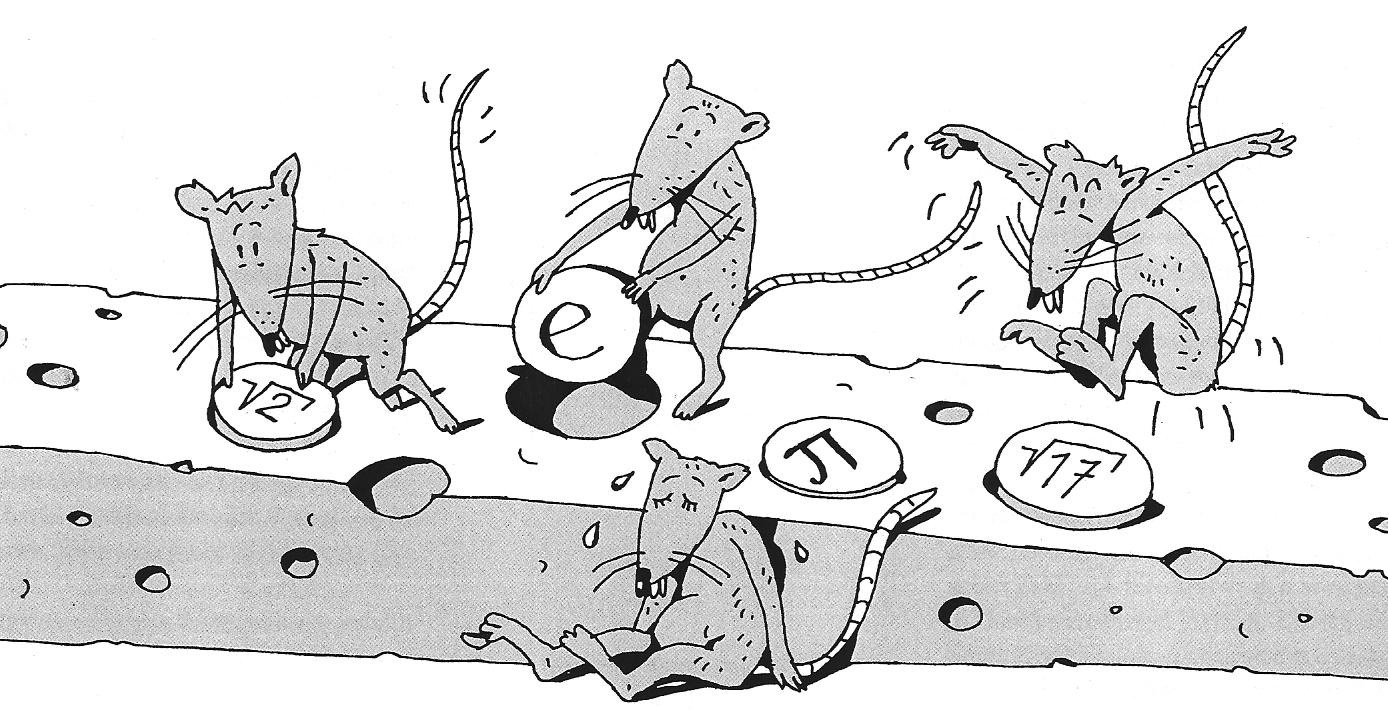
\includegraphics[width=0.618\textwidth]{pictures/irratzahlen}}
\title{Zahlen}
\subtitle{I like primes!}
\author{}
\date{}
\lowertitleback{
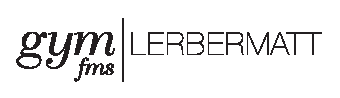
\includegraphics[height=1cm]{pictures/gymfmslerbermattlogo.eps}
\hfill%\copyright%
{\begin{tikzpicture}
  % Draw the rounded rectangle and clip the image to it
  \clip [rounded corners=5mm] (0,0) rectangle (1,1); % Adjust dimensions as needed
  \node at (0.5,0.5) {\includegraphics[width=1cm]{pictures/teacher_me_caricatur.png}}; % Adjust width and center image
\end{tikzpicture}}
}

\begin{document}
\maketitle
\tableofcontents
%\thispagestyle{empty}
\cleardoublepage
%\setcounter{page}{1}


\section{Natürliche Zahlen}
\subsection{Historisches}
\begin{quote}
Alles ist Zahl.
\end{quote}

\begin{wrapfigure}{r}{0.382\textwidth}
\vspace{-22pt}
  \begin{center}
    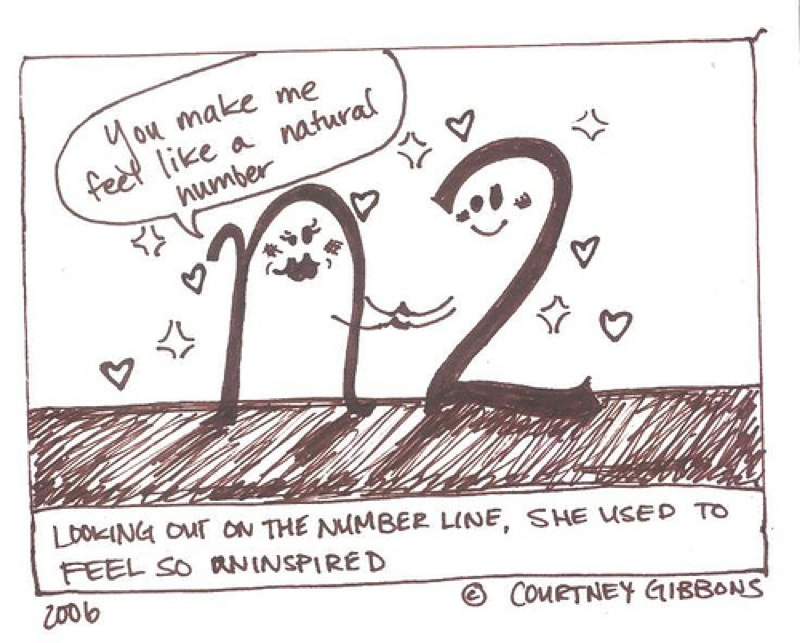
\includegraphics[width=0.38\textwidth]{pictures/zahln}
  \end{center}
%\caption{A gull}
\vspace{-22pt}
\end{wrapfigure}
Diese Aussage stammt von \textsc{Pythagoras}, dem berühmten griechischen Mathematiker und Philosophen, der um $\unit[550]{v.u.Z.}$ gelebt hat. In jungen Jahren soll er sich auf Anraten von \textsc{Thales} ($\unit[624-546]{v.u.Z.}$) auf eine langjährige Studienreise nach Ägypten begeben haben, um dort die vorhandenen Wissensschätze zu studieren. Nach \textsc{Pythagoras} sollte das menschliche Leben geordnet und harmonisch sein, wie es die Zahlenverhältnisse in der Natur offenbarten. Dieses Zahlenverständnis kommt im Satz \glqq Alles ist Zahl\grqq\ treffend zum Ausdruck und verdeutlicht, dass er die Zahlen als eine die gesamte Natur konstruierende Kraft betrachtete.

\subsection{Die Menge der natürlichen Zahlen}

Die natürlichen Zahlen $\mathbb{N}$ sind die seit Alters her beim Zählen verwendeten Zahlen.
Mit ihnen kann man eine Menge durchnummerieren. Die natürlichen Zahlen haben einen Anfang, die $1$, aber kein Ende. Das Symbol für Unendlich ist eine $\infty$.

Auf $\mathbb{N}$ können die Grundoperationen Addition und Multiplikation \definition{abgeschlossen} durchgeführt werden. Das heisst, dass auch das Ergebnis einer solchen Operation wieder eine natürliche Zahl ist.

Die Null gehört für uns nicht zu den natürlichen Zahlen. Wird $\mathbb{N}$ aber mit der Zahl Null erweitert, schreiben wir $\mathbb{N}_0$.

Zur Darstellung der natürlichen Zahlen eignet sich der \definition{Zahlenstrahl}.

\begin{center}
\scalebox{1.3}{
\begin{tikzpicture}[line cap=round,line join=round,>=triangle 45,x=0.8cm,y=0.4cm]
\draw[->,color=black] (-3.68,0) -- (6,0);
\foreach \x in {-3,-2,-1,0,1,2,3,4,5}
\draw[shift={(\x,0)},color=darkblue] (0pt,2pt) -- (0pt,-2pt) node[below] {\footnotesize $\x$};
\draw[color=black] (5.6,0.2) node [anchor=south west] {$\mathbb{R}$};
%\draw[color=black] (0pt,-10pt) node[right] {\footnotesize $0$};
\clip(-3.68,-1.32) rectangle (5.36,1.56);
\end{tikzpicture}
}
\end{center}

Eine saubere Fundierung der natürlichen Zahlen gelang im $\unit[19.]{Jahrhundert}$. Ein bedeutender Beitrag dazu stammte von \textsc{Georg Cantor}, dem die Einbindung des Unendlichen, $\infty$, gelang.
\marginnote{
\qrcode{
https://www.youtube.com/watch?v=qIfY1jMqjqY}
}
Er schuf mit der Mengenlehre ein Fundament, in dem einerseits die natürlichen Zahlen sicher eingebettet sind, aber auch der Begriff des Unendlichen nicht mit ihnen in  Widerspruch gerät.

\begin{uebenv}{johnvonneumann}
    \textsc{John von Neu\-mann} definierte die natürlichen Zahlen $\mathbb{N}_0$, wobei wir hier die Null dazu zählen, auf mengen\-theo\-re\-tischer Basis rekursiv wie folgt. Man be\-ginnt mit der leeren Menge, $\{\;\}$. Die folgende Menge bestehe aus der Menge, die alle vorangegangenen Mengen als Elemente enthält. Formaler: Der Nachfolger der Menge $\mathbb{M}$ ist $\mathbb{M}'=\mathbb{M}\cup\{\mathbb{M}\}$. Fährt man so immer fort, kriegt man eine Liste der natürlichen Zahlen $\mathbb{N}_0$. Nämlich, wenn man die Anzahl Elemente der entsprechenden Menge $\mathbb{M}$ zählt, $\text{card}(\mathbb{M})$.

    \begin{enumerate}[a)]
        \item Sei also $0:=\{\;\}$. Wie schreibt sich dann die nächste natürliche Zahl $1$?
        \item Notieren Sie in dieser Schreibweise die ersten $4$ natürlichen Zahlen.
    \end{enumerate}
\end{uebenv}



\begin{uebenv}{peano}
    Die Axiome der natürlichen Zahlenmenge von \textsc{Giuseppe Peano} lauten wie folgt \cite{peanoaxiome}:
    \begin{enumerate}
        \item $1$ ist eine natürliche Zahl.
        \item Jede natürliche Zahl $n$ hat eine natürliche Zahl $n'$ als Nachfolger.
        \item $1$ ist kein Nachfolger einer natürlichen Zahl.
        \item Natürliche Zahlen mit gleichem Nachfolger sind gleich.
        \item Enthält eine Menge $\mathbb{X}$ die Zahl $1$ und mit jeder natürlichen Zahl $n$ auch stets deren Nachfolger $n'$, so enthält $\mathbb{X}$ bereits alle natürlichen Zahlen. (Ist $\mathbb{X}$ dabei selbst eine Teilmenge der natürlichen Zahlen, dann ist $\mathbb{X}$ gleich der Menge der natürlichen Zahlen.)
    \end{enumerate}
Überzeugen Sie sich davon, dass keines der fünf Axiome weggelassen werden darf. Lassen Sie dabei Axiom $5$ unberührt. Was passiert, wenn man eines der ersten vier Axiome weg lässt? Geben Sie Gegenbeispiele an.
\end{uebenv}



\subsection{Primzahlen}

Unter den natürlichen Zahlen gibt es solche, die jedem Divisionsversuch mit einem natürlichen Divisor, der zwischen $1$ und der Zahl selbst liegt, widerstehen. Solche --- in diesem Sinne teilerlose --- Zahlen werden Primzahlen genannt.

\begin{cdef}[Primzahl]
Eine Zahl, die genau zwei verschiedene, natürliche Teiler hat, heisst Primzahl.
\end{cdef}

Somit gehören die Zahlen
$$2,3,5,7,11,13,17,19,23,\dots$$
zu den Primzahlen.

\begin{bem}
Beachte, dass $1$ per Definition keine Primzahl ist!
\end{bem}

Primzahlen sind die Bausteine der natürlichen Zahlen. Dies besagt der folgende Satz, den ich gerne als Satz der DNA der natürlichen Zahlen bezeichne.

\begin{csatz}[DNA der natürlichen Zahlen]
Jede natürliche Zahl grösser $1$ lässt sich eindeutig als Produkt von Primzahlen darstellen.
\end{csatz}

\begin{proof}
Widerspruchsbeweis: Falls die Primfaktorzerlegung in $\mathbb{N}\setminus\{1\}$ nicht eindeutig wäre, dann gäbe es eine kleinste Zahl $n\in\mathbb{N}\setminus\{1\}$, die auf mindestens 2 Arten darstellbar wäre:
$$n=p_1\cdot\ldots\cdot p_r=q_1\cdot\ldots\cdot q_s.$$
Da $n$ das kleinste Beispiel ist, sind alle $p_i\neq q_j$ für alle $i,j$ in ihren Indexmengen. Ausserdem können wir OEdA annehmen, dass die Faktoren der Grösse nach sortiert seien (Wohlordnung von $\mathbb{N}$) und $p_1\neq q_1$ mit $p_1+1\leq q_1\leq\sqrt{n}$. Betrachte nun $m:=n-p_1q_1$ mit $\sqrt{n}<m<n$. Beachte, dass $m<n$ eine eindeutige Primfaktorzerlegung hat. Aus
$$m=p_1\cdot(p_2\cdot\ldots\cdot p_r-q_1)=q_1\cdot(q_2\cdot\ldots\cdot q_s-p_1)$$
folgt $p_1|(q_2\cdot\ldots\cdot q_s-p_1)$, also $p_1|(q_2\cdot\ldots\cdot q_s)$. Weil aber für Zahlen kleiner $n$ die Primfaktorzerlegung eindeutig ist, muss $p_1=q_j$ für ein $j\neq1$. Widerspruch zu $p_1\neq q_j$ $\forall j$.
\end{proof}

\begin{uebenv}{primfaktorzerlegung}
Zerlege die Zahlen $234600$ und $7571$ in ihre Primfaktoren.
\end{uebenv}




\subsubsection{Etwas Zahlentheorie}

Als Bausteine der Zahlen scheinen die Primzahlen offensichtlich wichtig zu sein.

\subsubsection{Sieb von Eratosthenes}

Der alexandrinische Bibliothekar, Mathematiker und Geograph  \textsc{Eratosthenes} ($\unit[276-194]{v.u.Z.}$), der als erster einen ausgezeichneten Wert für den Umfang der Erde ermittelt hat, kannte bereits ein einfaches Verfahren, um die Primzahlen schrittweise aus der Reihe der natürlichen Zahlen heraus zu filtern (das \definition{Sieb des Eratosthenes}).

Betrachten wir die Primzahlen kleiner $100$:

\begin{quote}
2, 3, 5, 7, 11, 13, 17, 19, 23, 29, 31, 37, 41, 43, 47, 53, 59, 61, 67, 71, 73, 79, 83, 89, 97
\end{quote}

Auffallend ist, dass die Primzahlen scheinbar zufällig über $\mathbb{N}$ verteilt sind. Zudem gibt es Primzahlen, die sich als Paar um eine einzige Zahl schmiegen, wie zum Beispiel $11$ und $13$, $17$ und $19$, $29$ und $31$ oder $59$ und $61$. Die von einem solchen \definition{Primzahlzwilling} eingeschlossene Zahl besitzt immer viele Teiler, auf jeden Fall den Teiler $6$.

\begin{uebenv}{primzahlzwillinge}
Beweise, dass die Zahl zwischen einem Primzahlzwilling, $(p|p+2)$ mit $p$, $p+2$ beide prim, durch $6$ teilbar ist.
\end{uebenv}



\begin{uebenv}{primzahldrillinge}
    Gibt es \definition{Primzahldrillinge}, also Zahlentrippel mit $p$,$p+2$ und $p+4$ alle prim?
\end{uebenv}

Es ist übrigens nicht bekannt, ob es endlich oder unendlich viele Primzahlzwillinge gibt.

Die Lücken, das heisst die Anzahl der nichtprimen Zahlen zwischen zwei Primzahlen, sind in der Reihe der natürlichen Zahlen ganz verschieden gross. Je weiter in der Zahlenreihe fortgeschritten wird, um so grössere, derartige Lücken --- nebst den kleinsten --- treten auf.



\subsubsection{Dichte von Primzahlen}

Deutlich ist, dass die Primzahlen im allgemeinen mit wachsenden Zahlenwerten weniger häufig auftreten. Aber auch diese Gesetzmässigkeit wird durchbrochen. So finden wir in den ersten Hunderter-Blöcken die folgenden Anzahlen Primzahlen:

\begin{center}
\begin{tabular}{rrr}
\rowcolor{Gray}\spaltenheight $1$ bis $100$ & $101$ bis $200$ & $201$ bis $300$\spaltensep
\rowcolor{lightyellow}\spaltenheight $25$ & $21$ & $16$\spaltensep
\rowcolor{Gray}\spaltenheight $301$ bis $400$ & $401$ bis $500$ & $501$ bis $600$\spaltensep
\rowcolor{lightyellow}\spaltenheight $16$ & $17$ & $14$\spaltensep
\rowcolor{Gray}\spaltenheight $601$ bis $700$ & $701$ bis $800$ & $801$ bis $900$\spaltensep
\rowcolor{lightyellow}\spaltenheight $16$ & $14$ & $15$\spaltensep
\rowcolor{Gray}\spaltenheight $901$ bis $1000$ & &\spaltensep
\rowcolor{lightyellow}\spaltenheight $14$ & &\spaltensep
\end{tabular}
\end{center}

Das erste Tausend weist also $168$ Primzahlen auf, was etwa $\nicefrac{1}{6}$ aller natürlichen Zahlen dieses Intervalls entspricht. In den ersten $3000$ finden sich etwa $\nicefrac{1}{7}$, und unter den ersten $10\,000$ treffen wir auf rund $\nicefrac{1}{8}$. Die Dichte nimmt also scheinbar ab.
\marginnote{
\qrcode{
https://www.youtube.com/watch?v=Lg9GPyNOmSE}
}
Ist die Menge der Primzahlen also endlich? Gibt es eine grösste Primzahl?
Der \emph{indirekte} Beweis der Antwort auf diese Frage, lieferte schon \textsc{Euklid}\footnote{griechischer Mathematiker um $\unit[350]{v.u.Z.}$.}
 
\begin{uebenv}{unendlichvieleprimes}
    Zeige, dass es unendlich viele Primzahlen gibt.
\end{uebenv}



 
\begin{figure}
\begin{center}
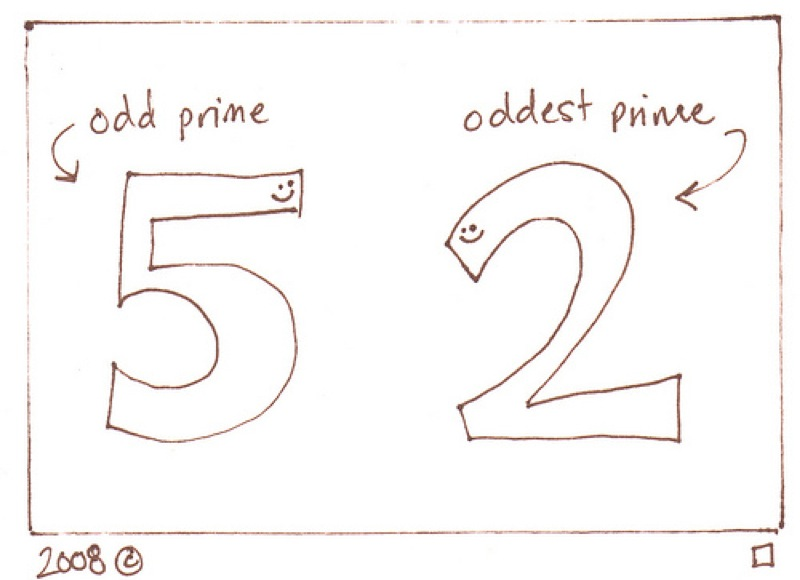
\includegraphics[width=0.3828\textwidth]{pictures/primzahl}
\caption{Seltsamste Primzahl}
\end{center}
\end{figure}
 
\subsubsection{Der grosse Satz von Fermat}
 
Ein um die Jahrtausendwende gelöstes zahlentheoretisches Problem, das sogar in der Presse seinen Niederschlag fand, ist der grosse Satz von Fermat.

\begin{csatz}[Grosser Fermat'scher Satz]
Für $,x,y,z,n\in\mathbb{N}$ mit $n>2$, $y$, $z$ und $n>2$ ist Gleichung
$$x^n+y^n=z^n$$
nicht erfüllbar.
\end{csatz}

\textsc{Fermat}\footnote{französischer Mathematiker (1601--1665)} selbst hinterliess auf dem Blattrand einer Manuskriptseite die Notiz:

\begin{quote}
    Wenn $n$ eine Zahl grösser als $2$ bedeutet, so gibt es keine positiven ganzen Zahlen $a$, $b$ und $c$, so dass $a^n+b^n=c^n$ wäre. Ich habe dafür einen wahrhaft wundervollen Beweis gefunden, der aber auf diesem Rande keinen Platz findet!
\end{quote}

    Für $n=2$ entspricht die oben genannte Gleichung dem Satz des Pythagoras, und der hat natürlich Lösungen. Man spricht in diesem Zusammenhang von \definition{pythagoräischen Zahlentripeln}.

\subsubsection{Primzahlen im Internet}

Die Suche nach schnellen Verfahren zum Auffinden von Primzahlen dauert bis zum heutigen Tag an; und das nicht nur aufgrund des Reizes, den sie seit jeher auf die Menschen ausgeübt haben. Über zweitausend Jahre lang wusste man keinen praktischen Nutzen aus dem Wissen über die Primzahlen zu ziehen. Dies änderte sich allerdings schlagartig mit dem Aufkommen des elektronischen Datenverkehrs, als Primzahlen zum Verschlüsseln von Informationen eine zentrale Rolle zu spielen begannen.

Die Güte einer Geheimsprache besteht einerseits darin, Botschaften ohne grossen Aufwand in Geheimschrift umschreiben (chiffrieren) zu können, andererseits darin, die Schwierigkeit für Uneingeweihte eine geheime Botschaft zu knacken (dechiffrieren), ins Unermessliche zu steigern. Solch asymmetrische Eigenschaften trifft man beim Rechnen mit Primzahlen an:

\begin{quote}
Es ist relativ einfach, das Produkt von zwei grossen Primzahlen zu berechnen, aber nahezu unmöglich, dieses Produkt wieder in seine Faktoren zu zerlegen.
\end{quote}

Das Verschlüsseln einer Botschaft läuft heute tatsächlich auf die Multiplikation zweier sehr grosser Primzahlen hinaus, während das Entschlüsseln im Wesentlichen aus dem Faktorisieren dieses Produkts besteht (ausprobieren).
Bis dato (\the\year) hat man noch keinen schnellen Algorithmus zur Faktorisierung eines Produkts zweier grosser Zahlen gefunden. Ja, man weiss sogar nicht einmal, ob ein solcher überhaupt existiert.

\subsection{Übungen zu $\mathbb{N}$ und Primzahlen}

\begin{uebenv}{primzahlformel}
Was taugen die folgenden Formeln als Primzahlerzeuger? Dabei steht stets $p$ für eine Primzahl und $n$ für eine natürliche Zahl.

    \begin{enumerate}[a)]
        \item $z_a=2^p-1$
        \item $z_b=2^p+1$
        \item $z_c=n^2-n+41$
        \item $z_d=n^2-79n+1601$
    \end{enumerate}
\end{uebenv}



\begin{uebenv}{goldbach}
Wähle $5$ gerade Zahlen zwischen $3$ und $1000$. Versuche jeder dieser Zahlen als Summe von zwei Primzahlen darzustellen (Stichwort Goldbach'sche Vermutung).
\end{uebenv}



\begin{figure}
    \begin{center}
        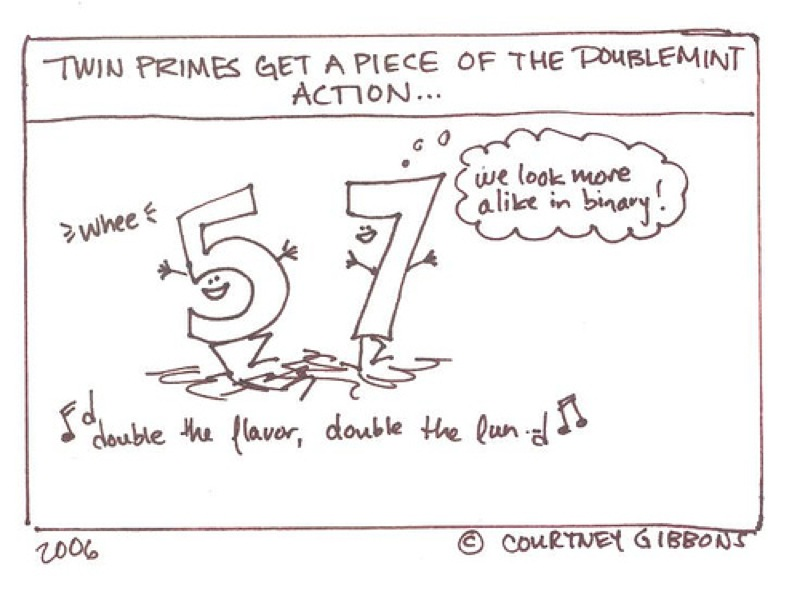
\includegraphics[width=0.382\textwidth]{pictures/primzahlzwillinge}
        \caption{Primzahlzwillinge}
    \end{center}
\end{figure}

\begin{uebenv}{primzahllcken}
Es gibt \glqq Primzahllücken\grqq{} beliebiger Grösse. Man definiert für $n\in\mathbb{N}$ den Ausdruck $n!:=1\cdot2\cdot3\cdot\dots\cdot n$ und sagt \glqq $n$ Fakultät\grqq.
    \begin{enumerate}[a)]
        \item Sind unter den Zahlen $5!+1$, $5!+2$, $5!+3$, $5!+4$ und $5!+5$ Primzahlen?
        \item Welche der Zahlen $47!+1, 47!+2, 47!+3,\dots,47!+47$ sind sicher nicht prim?
        \item Formulieren Sie nun allgemein für $n\in\mathbb{N}$ welche der Zahlen $n!+1,n!+2,\dots,n!+n$ sicher nicht prim sind.
    \end{enumerate}
\end{uebenv}




\begin{uebenv}{teilen}
    Nimm eine dreistellige Zahl und notiere sie zweimal hintereinander, so dass eine sechstellige Zahl entsteht. Teile diese Zahl nacheinander durch $7$, $11$ und $13$.
    \begin{enumerate}[a)]
        \item Was fällt auf?
        \item Kannst du deine Vermutung begründen?
    \end{enumerate}
\end{uebenv}




\begin{uebenv}{vielfache}
Zeige, dass die Summe von vier aufeinander folgenden natürlichen Zahlen niemals ein Vielfaches von $4$ sein kann.
\end{uebenv}




\begin{uebenv}{vierersumme}
Vier aufeinanderfolgende natürliche Zahlen werden miteinander multipliziert und zum Produkt $1$ addiert.
\begin{enumerate}[a)]
    \item Stelle einige konkrete Berechnungen an.
    \item Stelle eine Vermutung auf und versuche, diese zu beweisen.
\end{enumerate}
\end{uebenv}




\begin{uebenv}{quadratzahlen}
Suche Quadratzahlen, welche bei der Division durch $3$ den Rest $2$ lassen. Solltest du keine derartige Zahl finden, so versuche zu beweisen, dass es keine Quadratzahl gibt, die bei der Division durch $3$ den Rest $2$ lässt.
\end{uebenv}




\subsection{ggT und kgV}

Primfaktorzerlegungen spielen auch beim Bestimmen des \definition{ggT} (grösster gemeinsamer Teiler) und des \definition{kgV} (kleinstes gemeinsames Vielfaches) zweier natürlicher Zahlen $a$ und $b$ eine wichtige Rolle.

\begin{uebenv}{gcdandlcm}
Bestimme das kgV und den ggT der Zahlen $153900$ und $180600$.
\end{uebenv}




\subsubsection{Euklid'scher Algorithmus}

Um den ggT zweier Zahlen $a$ und $b$ zu finden, gelangt man häufig mit dem \regel{Euklid'schen Algorithmus} am schnellsten zum Ziel. Als Beispiel betrachten wir nochmals die beiden Zahlen $153900$ und $180600$, dividieren zuerst die grössere durch die kleinere und bestimmen danach den Rest, der entsteht.
\marginnote{
\qrcode{
https://www.youtube.com/watch?v=m8_OtbfpBnY}
}
In einem zweiten Schritt wird die kleinere Zahl durch den erhaltenen Rest geteilt und der dadurch resultierende neue Rest bestimmt, etc\dots.

Zwischen dem ggT und dem kgV besteht der folgende Zusammenhang.

\begin{csatz}[Produktsatz]
$$a\cdot b=\text{ggT}(a,b)\cdot\text{kgV}(a,b)$$
\end{csatz}

\begin{proof}
Für das kgV nimmt man jeweils die maximal vorkommende Anzahl der Primfaktoren aus beiden Zahlen, für den ggT jeweils die minimale Anzahl der gemeinsamen Primfaktoren. Kommt also ein Primfaktor nur in einer der Zahlen vor, so wird er wegen des kgVs verwendet und taucht im ggT nicht auf. Kommt ein Faktor in beiden Zerlegungen vor, so wird er in seiner maximalen Anzahl wegen des kgVs genommen und wegen seiner minimalen Anzahl für den ggT.
\end{proof}

\begin{uebenv}{euklidscheralg}
    Zeige, dass der Euklid'sche Algorithmus stets den ggT der beiden Zahlen liefert.
\end{uebenv}



\begin{uebenv}{euklidbsp}
Bestimme den ggT und das kgV der Zahlen $5544$ und $4410$ mit dem euklidschen Algorithmus und dem letzten Satz.
\end{uebenv}

\clearpage

\subsection{Notizen zu den Übungen}

\begin{lsg}{johnvonneumann}
    \begin{enumerate}[a)]
        \item Die $1$ ist dann die Menge mit der $0=\{\;\}$, also $1=\{\{\;\}\}$. Beachten Sie, dass die leere Menge kein Element enthält, jedoch die $1$ die leere Menge enthält, also ein Element.
        \item Die ersten vier natürlichen Zahlen lauten: $1=\{\{\;\}\}$, $2=\{\{\;\},\{\{\;\}\}\}$, $3=\{\{\;\},\{\{\;\}\},\{\{\;\},\{\{\;\}\}\}\}$, $4=\{\{\;\},\{\{\;\}\},\{\{\;\},\{\{\;\}\}\},\{\{\;\},\{\{\;\}\},\{\{\;\},\{\{\;\}\}\}\}\}$
    \end{enumerate}
\end{lsg}
\begin{lsg}{peano}
    Lässt man beispielsweise 1 weg, so fehlt das Charakteristikum \glqq natürliche Zahl sein\grqq und kann nicht weiter vererbt werden. Fehlt Axiom 2, so hätte nicht jede natürliche Zahl einen Nachfolger. Damit wäre es nicht möglich, alle (unendlich viele) natürlichen Zahlen zu erzeugen. Beispielsweise wäre $\mathbb{N}=\{1,2,3\}$ möglich.
    Fehlt Axiom 3, so könnte man einen Zirkelschluss bilden, indem man beispielsweise $1$ als Nachfolger der $2$ nimmt: $1,2,1,2,1,2,1,\dots$. Verzichtet man auf Axiom $4$, dann wäre es denkbar, dass zwei verschiedene natürliche Zahlen $n\neq m$ den gleichen Nachfolger hätten. Zum Beispiel: $1,3,2,3,2\dots$.
\end{lsg}
\begin{lsg}{primfaktorzerlegung}
$234600=2^3\cdot3\cdot5^2\cdot17\cdot23$, $7571=67\cdot113$
\end{lsg}
\begin{lsg}{primzahlzwillinge}
Für $(3\mod5)$ stimmt die Aussage nicht. Lassen wir also diesen Fall ausser betracht.

Da $2$ die einzige gerade Primzahl ist, muss die Zahl zwischen einem Primzahlzwilline gerade sein. Betrachte für $k\in\mathbb{N}$ grösser als $3$ die Kette
$$k-2\quad k-1\quad k\quad k+1\quad k+2\quad k+3.$$
Damit werden für $k\in\mathbb{N}$ alle natürlichen Zahlen durchlaufen. $k-2$ und $k$, sowie $k$ und $k+2$ und $k+1$, $k+3$ können keine Primzahlzwillinge sein. Denn gälte $k\mod3\equiv1$ dann $k-2\mod3\equiv2$, also einer von beiden gerade bzw. $k+2\mod3\equiv0$, also durch $3$ teilbar. Analog für $k\mod3\equiv2$. Also kommt als Primzahlzwilling in dieser Kette nur $(k-1\mid p+1)$ in Frage. $k-1\mod3\equiv1$ kann nicht sein, da dann $k+1\mod3\equiv0$ wäre. Also muss $k-1\mod3\equiv2$ und damit $k\mod3\equiv0$. Also ist $k$ durch $2$ und durch $3$ teilbar, also durch $6=2\cdot3$.
\end{lsg}
\begin{lsg}{primzahldrillinge}
    Es gibt nur das Tripel $(3|5|7)$. Denn jedes weitere Tripel würde ungerade Zahlen enthalten, wobei sicher eine davon durch $3$ teilbar wäre, da jede dritte ungerade Zahl durch $3$ teilbar ist.

    Man kann dies auch formal einsehen:
    \begin{proof}
        Wäre $(p|p+2|p+4)$ mit $p>3$ ein weiteres Tripel, so dürfte $p$ nicht durch $3$ teilbar sein. Es gälte also $p\mod{3}\equiv1$ oder $p\mod{3}\equiv2$. Sei $p\mod{3}\equiv1$, dann ist aber $p+2\mod{3}\equiv0$ durch $3$ teilbar, also keine Primzahl. Gälte $p\mod{3}\equiv2$, so wäre $p+4\mod{3}\equiv0$ durch $3$ teilbar. Somit ist $(3|5|7)$ der einzige Primzahldrilling.
    \end{proof} 
\end{lsg}
\begin{lsg}{unendlichvieleprimes}
\begin{proof}
        Gegenannahme: Es gebe endlich viele Primzahlen und daher gebe es eine grösste, die wir $p$ nennen. Wir betrachten die Menge dieser endlich vielen Primzahlen
        $$\{2,3,5,7,11,\dots,p\}.$$ Wir basteln daraus die Zahl
        $$2\cdot3\cdot5\cdot7\cdot11\cdot\dots\cdot p+1=:z.$$
        Diese Zahl $z\in\mathbb{N}$ ist sicher grösser als $p$ und sie ist auch prim. Denn beispielsweise hat man $z\div 7=2\cdot3\cdot5\cdot11\cdot\dots\cdot p+1$, d.h. $z=7\cdot2\cdot3\cdot5\cdot11\cdot\dots\cdot p+1$ hat bei Division mit $7$ Rest $1$. Und dies gilt analog für alle Primzahlen in unserer Menge
        $$\{2,3,5,7,11,\dots,p\}.$$ Dies widerspricht der Annahme, dass $p$ die grösste Primzahl sei, denn $z>p$ ist prim. Also muss das Gegenteil unserer Annahme gelten: Es gibt unendlich viele Primzahlen.
    \end{proof}
\end{lsg}
\begin{lsg}{primzahlformel}
\begin{enumerate}[a)]
    \item $p=3$ liefert $4$.
    \item $p=2$ liefert $8$.
    \item $n=41$ liefert sicher keine Primzahl, weil $z_c(41)=41^2$.
    \item Für $n=80$ ist $z_d(80)=41^2$
\end{enumerate}
\end{lsg}
\begin{lsg}{goldbach}
Beispiele sind $4=2+2$, $6=3+3$, $8=3+5$, $10=3+7$. Beachte, dass die Zerlegung nicht eindeutig sein muss. Beispielsweise ist $10=3+7=5+5$ oder $20=3+17=7+13$.

    Bis dato (\the\year) konnte die Goldbach-Vermutung nicht bewiesen werden.
    
    Sidenote: Dem Russen \textsc{Vinogradov} gelang mittels statistischer Methoden über die Primzahlen um die Jahrhundertwende der Beweis, dass sich jede \glqq genügend\grqq{} grosse, ungerade Zahl als Summe von drei Primzahlen schreiben lässt.
\end{lsg}
\begin{lsg}{primzahllcken}
\begin{enumerate}[a)]
        \item $5!+1=121=11^2$, $5!+2=122$ ist gerade, $5!+3=123=3\cdot41$, $5!+4$ ist gerade, $5!+5=125=5^3$ sind alle nicht prim.
        \item Für $47!+1$ ist ohne Hilfsmittel aufwändig zu beurteilen, ob sie prim ist oder nicht. Hingegen $47!+2=1\cdot2\cdot3\cdot\dots\cdot47+2=2\cdot(1\cdot3\cdot\dots\cdot47+1)$. Analog $47!+3=1\cdot2\cdot3\cdot\dots\cdot47+3=3\cdot(1\cdot2\cdot4\cdot\dots\cdot47+1)$. Das heisst, alle Zahlen $47!+2$, $47!+3$, $\dots$, $47!+47$ sind sicher nicht prim.
        \item Für $n\in\mathbb{N}$ kann man im Allgemeinen wie oben nicht eruieren, ob $n!+1$ prim ist oder nicht. Andererseits sind $n!+2=2\cdot(3\cdot4\cdot\dots\cdot n+1$ bis $n!+n=n\cdot(2\cdot3\cdot\dots\cdot(n-1)+1)$ wegen der hier gezeigten Faktorisierung sicher nicht prim. Also gibt es Primzahllücken beliebiger Grösse.
    \end{enumerate}
\end{lsg}
\begin{lsg}{teilen}
 \begin{enumerate}[a)]
        \item Man kriegt wieder diejenige dreistellige Zahl, die man sich ausgedacht hat.
        \item Wenn man durch die Werte $7$, $11$ und $13$ in Folge teilt, so entspricht dies einer Division mit $7\cdot11\cdot13=1001$. Eine dreistellige Zahl multipliziert mit $1001=1000+1$ erzeugt den Effekt von zweimal hintereinander schreiben; zum Beispiel $123\cdot1001=123123$.
    \end{enumerate}
\end{lsg}
\begin{lsg}{vielfache}
In der Tat ist für beliebig gewähltes $n\in\mathbb{N}$ die Summe von vier aufeinander folgenden natürlichen Zahlen $n+(n+1)+(n+2)+(n+3)=4n+6=4\cdot(n+1)+2$ immer $(n+(n+1)+(n+2)+(n+3))\mod{4}\equiv2$, hat also Rest $2$ bei Division mit $4$.
\end{lsg}
\begin{lsg}{vierersumme}
 \begin{enumerate}[a)]
        \item Beispielsweise hat man $1\cdot2\cdot3\cdot4+1=25=5^2$, $2\cdot3\cdot4\cdot5+1=121=11^2$ oder $10\cdot11\cdot12\cdot13+1=17\,161=131^2$.
        \item Für $n\in\mathbb{N}$ beliebig berechnet man
        \begin{align*}
        n(n+1)(n+2)(n+3)+1 &=(n^2+n)(n^2+5n+6)+1\\
        &=n^4+6n^3+11n^2+6n+1\\
        &=(n^2+3n+1)(n^2+3n+1)\\
        &=(n^2+3n+1)^2.
        \end{align*}
        Also ist dies immer eine Quadratzahl, da ja $n^2+3n+1\in\mathbb{N}$.
    \end{enumerate}
\end{lsg}
\begin{lsg}{quadratzahlen}
Man kriegt bei der Division durch $3$ nie den Rest $2$. Einige Beispiele: $1^2\mod{3}\equiv1$, $2^2\mod{3}\equiv1$, $3^2\mod{3}\equiv0$ oder $4^2\mod{3}\equiv1$.

        In der Tat:
        \begin{proof}
            Betrachten Sie für $n\in\mathbb{N}$ die Kette
            $$3n-2,3n-1,3n,$$
            welche für $n\in\mathbb{N}$ alle natürlichen Zahlen durchläuft. Die Quadrate $(3n-2)^2=9n^2-12n+4=3\cdot (3n^2-4n+1)+1$ und $(3n-1)^2=9n^2-6n+1=3\cdot(3n^2-2n)+1$ haben offensichtlich Rest $1$ bei Division mit $3$. Das Quadrat $9n^2=3\cdot3n^2$ hat Rest $0$ bei Division durch $3$. Daher kann keine Quadratzahl bei Division durch $3$ Rest $2$ haben.
        \end{proof}
\end{lsg}
\begin{lsg}{gcdandlcm}
Es ist
\begin{align*}
    153\,900 &= 2^2\cdot3^4\cdot5^2\cdot19\\
    180\,600 &= 2^3\cdot3\cdot5^2\cdot7\cdot43
\end{align*}
und daher $\text{ggT}(180\,600, 153\,900)=2^2\cdot3\cdot5^2$ und $\text{kgV}(180\,600, 153\,900)=2^3\cdot3^4\cdot5^2\cdot7\cdot19\cdot43$.
\end{lsg}
\begin{lsg}{euklidscheralg}
    OEdA sei $a\geq b$. Wir zeigen zuerst, dass sich der ggT über eine \glqq Algorithmusrunde\grqq{} nicht ändert. Der Algorithmus läuft so:
    \begin{align*}
        a &= q_1\cdot b+r_1\\
        b &= q_2\cdot r_1+r_2\\
        r_1 &= q_3\cdot r_2+r_3\\
        &\vdots\\
        r_{n-1} &= q_{n+1}\cdot r_n+0 
    \end{align*}
    Es ist $\text{ggT}(a,b)\leq \text{ggT}(b,r_1)=\text{ggT}(b,a-q_1 b)$: Setze $\text{ggT}(a,b)=:t$. Klar $t|a$ und $t|b$, d.h. $\exists k,l\in\mathbb{Z}$ mit $a=kt$ und $b=lt$. Es folgt $a-q_1 b=kt-q_1 lt=t(k-q_1l)$, also teilt $t$ $a-q_1 b$. Somit gilt $\text{ggT}(b,a-q_1b)\leq \text{ggT}(a,b)$. Sei umgekehrt $\text{ggT}(b,a-q_1b)=:u$, also $b=ku$ und $a-q_1b=lu$. Es folgt $a=lu-q_1b=lu-q_1ku=u(l-ku)$, also ist $u$ ein Teiler von $\text{ggT}(a,b)$, d.h. $ \text{ggT}(a,b)\leq\text{ggT}(b,a-q_1b)$. Insgesamt also $ \text{ggT}(a,b)=\text{ggT}(b,a-q_1b)$.

    Weil im letzten Schritt $\text{ggT}(r_{n-1},r_n)=\text{ggT}(r_n,0)=r_n$ ist $\text{ggT}(a,b)=r_n$, also gleich dem letzten, nichttrivialen Rest.
\end{lsg}
\begin{lsg}{euklidbsp}
\begin{align*}
    5544 &= 4410\cdot1+134\\
    4410 &= 134\cdot32+122\\
    134 &= 122\cdot1+12\\
    122 &= 12\cdot10+2\\
    12 &= 2\cdot6+0
\end{align*}
Der ggT ist also $2$.
\end{lsg}

\clearpage

\section{Die ganzen Zahlen}
\subsection{Die negativen Zahlen}
\subsubsection{Historisches}

\begin{wrapfigure}{r}{0.382\textwidth}
\vspace{-22pt}
  \begin{center}
    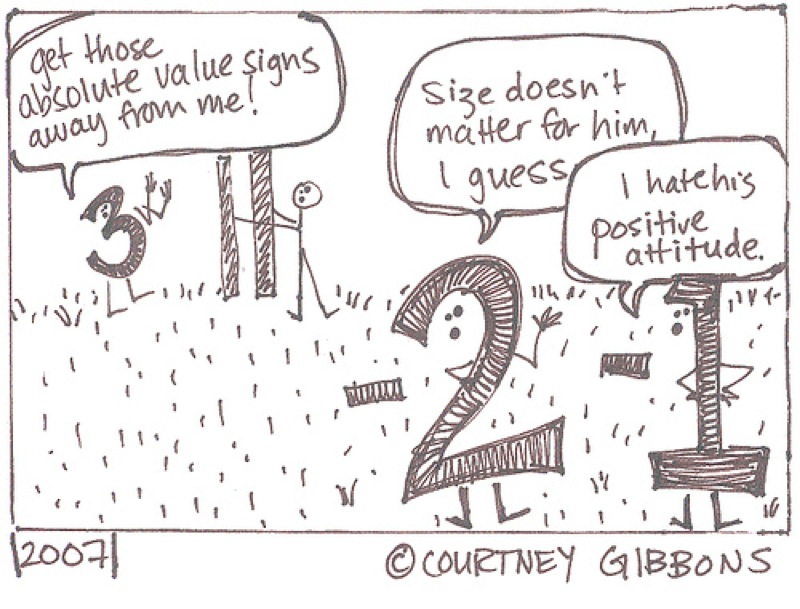
\includegraphics[width=0.38\textwidth]{pictures/negative}
  \end{center}
%\caption{Positive Attitude}
\vspace{-22pt}
\end{wrapfigure}
Der indische Mathematiker und Astronom \textsc{Brahmagupta} (598-630) erkannte als einer der ersten das Wechselspiel von Zahlzeichen, indem er Regeln für das Teilen von Zahlen aufstellte: \glqq Positiv geteilt durch positiv oder negativ geteilt durch
negativ gibt positiv. Positiv geteilt durch negativ oder negativ geteilt durch positiv gibt negativ.\grqq

In Europa erlaubte erst \textsc{Fibonacci} (1180-1241) in seiner Finanzmathematik negative Zahlen und interpretierte sie korrekterweise als Schulden.

\subsubsection{Die Geschichte der Null}
Ein ähnlich schwieriger Stand wie die negativen Zahlen hatte die Zahl Null, die in Europa auf Ablehnung und
Unverständnis stiess: Null wurde mit nichts gleichgesetzt.

Im Anhang \ref{ap:null} ist ein Artikel von \textsc{Herbert Cerutti} abgedruckt, der im Februar 2002 im NZZ-Folio \emph{Total Digital} erschienen ist.

\begin{uebenv}{hilbertshotel}
    Hilberts Hotel ist ein Hotel mit unendlichen vielen, nummerierten Zimmern $(1,2,3,\dots)$. Der Portier ist mit allen Zimmern durch eine Gegensprechanlage verbunden. Aktuell sind alle unendlich vielen Zimmer besetzt.
    \begin{enumerate}[a)]
        \item Es kommt ein Besucher an und möchte gerne ein Zimmer zum Übernachten buchen. Kann der Portier eines offerieren?
        \item Nun kommen unendlich viele Besucher an, die jeweile je ein Zimmer für sich buchen möchte. Kann der Portier helfen?
    \end{enumerate}
\end{uebenv}

\begin{uebenv}{gleichmchtig}
    Haben $\mathbb{N}_0$ und $\mathbb{Z}$ gleich viele Elemente? Anders: Finde eine bijektive Abbildung $f:\mathbb{N}_0\longrightarrow\mathbb{Z}$?
    
    Zwei Mengen $\mathbb{A}$ und $\mathbb{B}$ heissen \definition{gleichmächtig} (haben gleich viele Elemente), falls es eine bijektive Abbildung $f:\mathbb{A}\longrightarrow\mathbb{B}$ gibt.
\end{uebenv}

\clearpage

\subsection{Notizen zu den Übungen}

\begin{lsg}{hilbertshotel}
    \begin{enumerate}[a)]
        \item Der Portier kann die unendlich vielen Gäste auffordern, ihr Zimmer zu verlassen und das Zimmer mit der um $1$ grösseren Nummer zu belegen. Also $1\rightarrow 2$, $2\rightarrow3$, $3\rightarrow4$ etc. Nun ist Zimmer Nummer $1$ frei. Als Funktion geschrieben: $f:\mathbb{N}\longrightarrow\mathbb{N}$, $f(n)=n+1$.
        \item Ja! Beispielsweise kann der Portier beantragen, dass alle Gäste ins Zimmer mit der doppelten so grossen Nummer einziehen; also $1\rightarrow 2$, $2\rightarrow4$, $3\rightarrow6$ etc. Dadurch werden alle Zimmer mit ungeraden Nummern, $1,3,5,\dots$, frei, und das sind unendlich viele. Formal notiert: $f:\mathbb{N}\longrightarrow\mathbb{N}$, $f(n)=2n$.
    \end{enumerate}
\end{lsg}
\begin{lsg}{gleichmchtig}
    Beispielsweise kann man alle geraden Zahlen auf die positiven Werte abbilden, $0$ auf $0$ und alle ungeraden Zahlen den negativen Werten zuordnen:
    $$f:\mathbb{N}_0\longrightarrow\mathbb{Z}, f(n)=\begin{cases}
    \frac{n}{2} & \text{falls $n$ gerade}\\
    -\frac{n+1}{2} & \text{falls $n$ ungerade}
    \end{cases}
    $$
\end{lsg}

\clearpage

\section{Rationale Zahlen}
\subsection{Normalbrüche}
\begin{wrapfigure}{r}{0.382\textwidth}
\vspace{-22pt}
  \begin{center}
    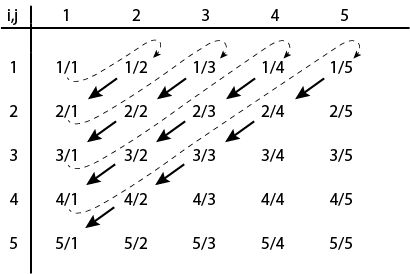
\includegraphics[width=0.38\textwidth]{pictures/Cantor}
  \end{center}
%\caption{Positive Attitude}
\vspace{-22pt}
\end{wrapfigure}
In der Menge der ganzen Zahlen $\mathbb{Z}$ kann die Division nicht immer
ausgeführt werden.
\bsp Die Rechnung $\,8\div 2\,$ liefert zwar wieder ein Element aus $\mathbb{Z}$ als Lösung (nämlich 4), aber $\;8\div 3\,$ ist in $\mathbb{Z}$ nicht mehr lösbar, denn $\,\frac{8}{3}=2.\overline{6}\notin\mathbb{Z}$. 
Wir suchen deshalb eine möglichst einfache Menge, welche die ganzen Zahlen enthält und welche die Division uneingeschränkt zulässt (ausser der Division durch 0, natürlich!).
Dies wird durch die Menge der rationalen Zahlen
$$\mathbb{Q} = \{\frac{p}{q}\mid p\in\mathbb{Z},\,q\in\mathbb{N}\}$$
gewährleistet.

\subsection{Dezimalbrüche}

Dezimalbrüche können in zwei Kategorien eingeteilt werden: Dezimalbrüche 
\begin{itemize}
	\item mit periodischer Dezimalbruchentwicklung (z.B. $1.5$ oder $3.5\overline{12}$)
	\item ohne periodische Dezimalbruchentwicklung (z.B. $0.10100100010\dots$)
\end{itemize}

Dezimalbrüche mit abbrechender Dezimalbruchentwicklung können unter der Menge Dezimalbrüche mit periodischer Dezimalbruchentwicklung subsummiert werden.
\marginnote{
\qrcode{
https://www.youtube.com/watch?v=GBgXSkXRu0g}
}

\begin{csatz}[Dezimaldarstellung rationaler Zahlen]
Jeder Normalbruch lässt sich in Form eines periodischen Dezimalbruchs schreiben, und umgekehrt.
\end{csatz}

Man muss zeigen, dass
\begin{itemize}
	\item jeder Normalbruch in einen periodischen Dezimalbruch und
	\item jeder periodische Dezimalbruch in einen Normalbruch umgewandelt werden kann.
\end{itemize}

Im Folgenden soll das Verfahren zur Umwandlung an ein paar Beispielen erläutert werden.

\subsection{Gedanken zu rationalen Zahlen}

\begin{uebenv}{abbrechendedezimalzahl}
Wie muss der Nenner eines Bruches beschaffen sein, damit die Dezimalbruchdarstellung abbrechend ist?
\end{uebenv}

\begin{uebenv}{periodenlnge}
Behauptung: Die Periodenlänge eines Bruches
$$\frac{1}{q}$$
wird nie länger als $q-1$.
\end{uebenv}

\begin{uebenv}{bruchunddezimal}

    \begin{enumerate}[a)]
        \item Verwandle den Bruch $\frac{3}{11}$ in eine Dezimalzahl.
        \item Bestimme den Bruch zur rationalen Zahl $0.1\overline{32}$.
    \end{enumerate}
\end{uebenv}

\clearpage

\subsection{Notizen zu den Übungen}

\begin{lsg}{abbrechendedezimalzahl}
Denken wir uns, wie man die Dezimaldarstellung mit schriftlicher Division erhält. Pro Divisionsschritt wird der jeweilige Rest ein Vielfaches von $10$ mit Primfaktorzerlegung $10=2\cdot5$ sein, weil wir ja im Dezimalsystem rechnen. Solch ein Rest wird somit genau dann ohne Divisionsrest teilbar sein, wenn in der Primfaktorzerlegung des Divisors (also dem Nenner) nur Primfaktoren $2$ oder $5$ vorkommen. Beispielsweise haben $\frac{1}{8}=\frac{1}{2^3}=0.125$, $\frac{1}{10}=\frac{1}{2\cdot 5}=0.1$ oder $\frac{1}{25}=\frac{1}{5^2}=0.04$ abbrechende Dezimaldarstellung.
\end{lsg}
\begin{lsg}{periodenlnge}
Sei $q\in\mathbb{N}$ beliebig. Bei der schriftlichen Division von $1$ mit $q$ können sicherlich nur Reste kleiner $q$ auftauchen; also die Reste $0,1,2,3,\dots,q-1$. Dies sind $q$ Stück. Im Falle vom Rest $0$ haben wir eine abbrechende Dezimaldarstellung. Also können alternierend höchstens die Reste $1,2,3,\dots,q-1$ vorkommen, und das sind $q-1$ Stück. Die Periodenlänge ist daher nie grösser als $q-1$.
\end{lsg}
\begin{lsg}{bruchunddezimal}
\begin{enumerate}[a)]
    \item \begin{align*}
        3\div11 &= 0.27\overline{27}\tag{Rest 3}\\
        30\div11 &=2\tag{Rest 8}\\
        80\div11 &=7\tag{Rest 3}
    \end{align*}
    \item \begin{align*}
        0.1\overline{32} &= x\\
        13.2\overline{32} &= 100x\\
        99x &= 13.1\\
        x &= \frac{13.1}{99}=\frac{131}{990}
    \end{align*}
\end{enumerate}
\end{lsg}

\clearpage

\section{Reelle Zahlen}

Es scheint, als sei die Zahlengerade durch die \glqq überall dicht\grqq\
liegenden rationalen Zahlen lückenlos besetzt, da sich zwischen zwei
noch so nahe beieinander liegenden rationalen Zahlen immer noch unendlich viele andere rationale Zahlen befinden. Diese Ansicht ist
falsch! Es gibt noch Lücken.

\subsection{Die Entdeckung der irrationalen Zahlen}
\begin{figure}
  \begin{center}
    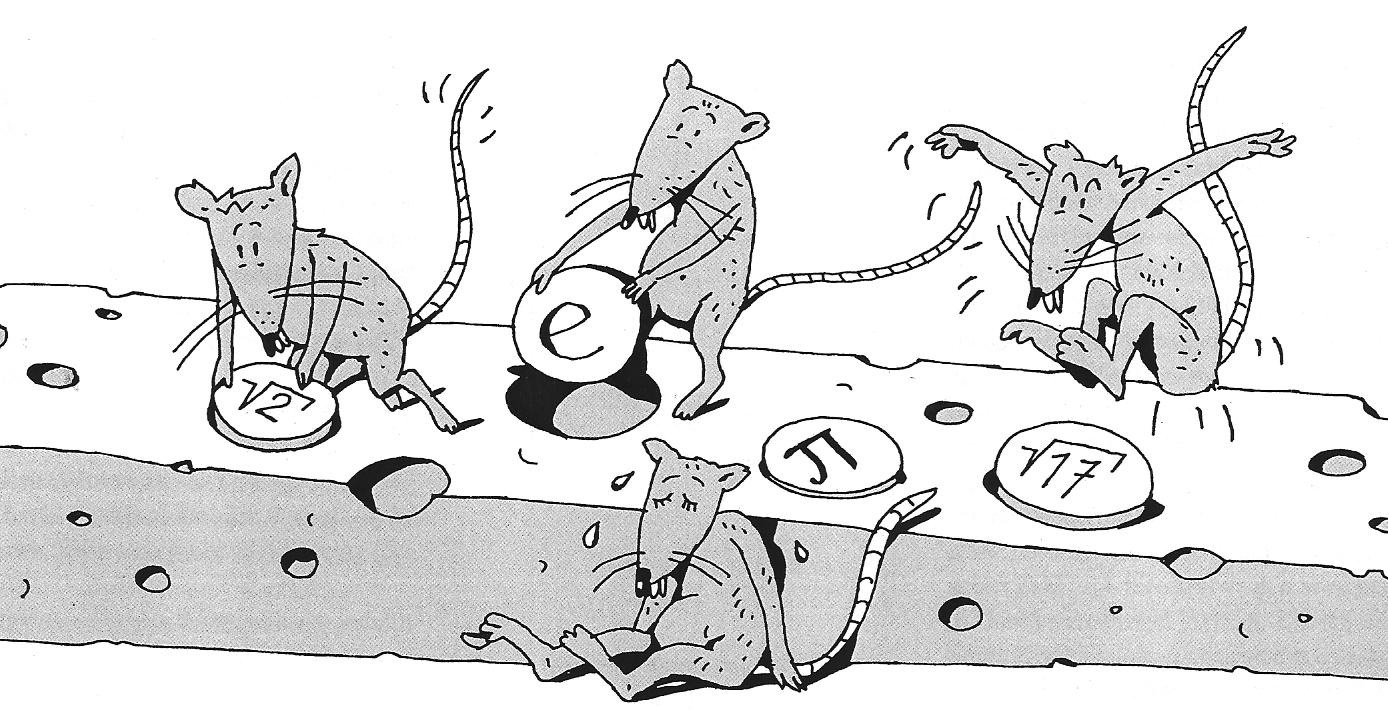
\includegraphics[width=0.382\textwidth]{pictures/irratzahlen}\hspace{2cm}
    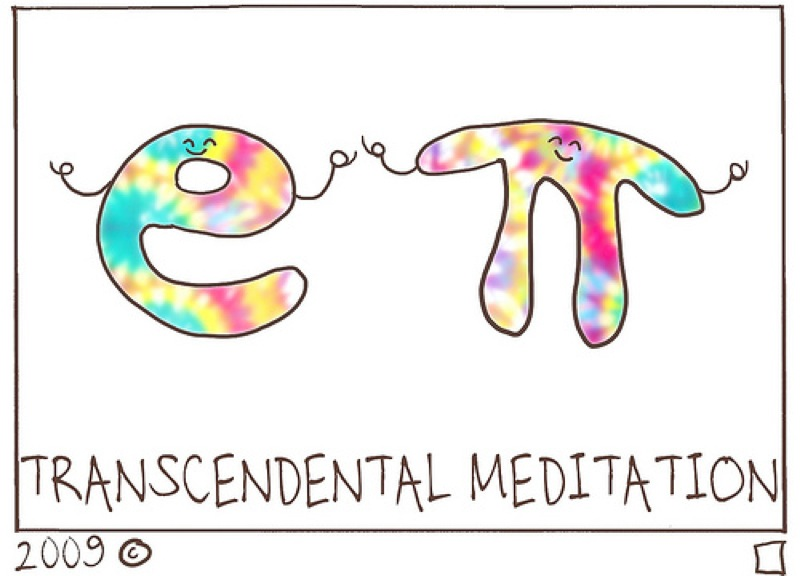
\includegraphics[width=0.382\textwidth]{pictures/transzendent}
  \end{center}
\caption{irrats and transcendents}
\end{figure}

In der goldenen Ära Griechenlands (bis ca.\ 400 v.u.Z.) galten unter den Gelehrten die natürlichen Zahlen und die Lehre ihrer Verhältnisse als das Mass aller Dinge. Die
Entdeckung von inkommensurablen Längen riss eine
grosse Kluft zwischen die Arithmetik, die diese  irrationalen Zahlen erschaffen konnte, und die Geometrie, die sie
nicht messen konnte. Ein Beispiel einer Zahl, die nicht durch ein
Verhältnis zweier ganzer Zahlen ausgedrückt werden kann, ist $\sqrt{2}$.

\begin{proof}
Indirekter
\marginnote{
\qrcode{
https://www.youtube.com/watch?v=_ONbuGauF9I}
}
Beweis hier über die Parität. Man könnte auch über die Eindeutigkeit der Primfaktorzerlegung argumentieren.

Sei $\sqrt{2}\in\mathbb{Q}$. Da $\sqrt{2}$ positiv, gibt es $a,b\in\mathbb{N}$ mit $\sqrt{2}=\frac{a}{b}$ vollständig gekürzt. Es folgt
\begin{align*}
    2 &= \frac{a^2}{b^2}\\
    2b^2 &= a^2
\end{align*}
und damit muss $a^2$ gerade sein. Wenn $a^2$ gerade ist, so muss auch $a$ gerade sein, da in $a^2$ mindestens zwei Faktoren $2$ vorkommen müssten. Betrachte weiter
\begin{align*}
    2b^2 &= a^2\\
    b^2 &= \frac{a^2}{2}=\frac{a}{2}\cdot a,
\end{align*}
was heisst, dass $b^2$ und damit $b$ gerade ist, denn das Produkt $\frac{a}{2}\cdot a$ ist immer gerade. Dies ist ein Widerspruch zur vollständig gekürzten Darstellung $\frac{a}{b}$, da dieser Quotient sicher noch mit $2$ gekürzt werden könnte!
\end{proof}

Die irrationalen Zahlen können nicht durch einen abbrechenden oder periodischen Dezimalbruch beschrieben
werden. Sie bilden zusammen mit den rationalen Zahlen die Menge der reellen Zahlen, $\mathbb{R}$. 

Neben den Wurzelzahlen $\sqrt{2}=1.41421\dots$, $\sqrt{3}=1.73205\dots$ etc.\ gehören Zahlen wie $\Pi=3.14159\dots$, die Euler'sche Zahl $\mathrm{e}=2.71828\dots$ und die Zahl des goldenen Schnitts $\Phi=1.61803\dots$ bzw. $\varphi=0.618\dots$
zu den berühmtesten irrationalen Zahlen.

\begin{bem}
Die reellen Zahlen werden manchmal auch in zwei  Mengen
aufgeteilt: In die \definition{algebraischen}, die als Nullstellen von
Polynomen mit ganzzahligen Koeffizienten aufgefasst werden können, also im Wesentlichen Wurzelausdrücke, und in die
\definition{transzendenten Zahlen}, das sind alle anderen. Während zum Ersteren die Zahl $\sqrt{2}$ und die des goldenen Schnitts $\phi$ gehören, sind die Zahlen $\pi$ und $\mathrm{e}$ transzendente Zahlen.
\end{bem}

\begin{uebenv}{primzahlwurzeln}
    Zeige, dass alle Primzahlwurzeln, das heisst $\sqrt{p}$ mit $p$ prim, irrational sind.
\end{uebenv}

\begin{uebenv}{primzahlwurzelalgebraisch}
    Zeige, dass jede Primzahlwurzel $\sqrt{p}$ algebraisch ist.
\end{uebenv}

\clearpage

\subsection{Notizen zu den Übungen}


\begin{lsg}{primzahlwurzeln}
    Sei $p\in\mathbb{N}$, $p$ prim. Gegenannahme $\sqrt{p}\in\mathbb{Q}$, das heisst $\exists a\in\mathbb{Z}, b\in\mathbb{N}$ so, dass
        $$\sqrt{p}=\frac{a}{b}.$$
        Es folgt
        \begin{align*}
            \sqrt{p} &= \frac{a}{b} \tag{$(\,)^2$}\\
            p &= \frac{a^2}{b^2}\tag{$\cdot b^2$}\\
            b^2\cdot p &= a^2 \label{eq:sqrtprimeW}
        \end{align*}
        In der Primfaktorzerlegung der Quadratzahlen $a^2$ und $b^2$ kommt jeder Primfaktor der Zerlegung sicher eine gerade Anzahl Mal vor. Der Primfaktor $p$ jedoch kommt in der Zahl $b^2\cdot p$ eine ungerade Anzahl Mal vor. Widerspruch zur Gleichheit in (\ref{eq:sqrtprimeW})!
\end{lsg}
\begin{lsg}{primzahlwurzelalgbraisch}
    Offensichtlich liefert $x^2-p=0$ die Behauptung.
\end{lsg}

\clearpage

\section{Dies \&\ Das zu Zahlenmengen}
\begin{uebenv}{zuordnung}
    Zu welcher kleinstmöglichen Zahlenmenge ($\mathbb{N}$, $\mathbb{Z}$, $\mathbb{Q}$ und $\mathbb{R}$) gehören die folgenden Zahlen?
    
        \begin{enumerate}[a)]
            \item $-5$
            \item $4.\overline{7}$
            \item $-\frac{5}{3}$
            \item $5.155155515555\dots$
            \item $\sqrt{121}$
            \item $\frac{15}{5}$
            \item $0$
            \item $-0.38\overline{27}$
        \end{enumerate}
\end{uebenv}



\begin{uebenv}{wahroderfalsch}
Sind diese Aussagen wahr oder falsch? Finde Beispiele oder Gegenbeispiele.
\begin{enumerate}[a)]
	\item Alle Differenzen von zwei natürlichen Zahlen sind natürliche Zahlen.
	\item Es gibt Quotienten von zwei natürlichen Zahlen, die irrational sind.
	\item Alle Quotienten von zwei rationalen Zahlen sind rationale Zahlen.
	\item Alle Wurzeln aus natürlichen Zahlen sind irrationale Zahlen.
    \item Das Quadrat einer irrationalen Zahl ist eine irrationale Zahl.
\end{enumerate}
\end{uebenv}



\begin{uebenv}{wahroderfalschzwei}
Sind diese Aussagen wahr oder falsch? Begründe.
	\begin{enumerate}[a)]
		\item Es gibt unendlich viele Zahlen zwischen 0.1 und $\dfrac{1}{9}$.
		\item $(1+\sqrt{2})$ ist eine irrationale Zahl, deren Quadrat irrational bleibt.
		\item Es gibt unendlich viele Zahlen, deren Wurzel gleich der Zahl selbst ist.
		\item Es gibt unendlich viele Zahlen, deren Wurzel grösser als die Zahl selbst ist.
	\end{enumerate}
\end{uebenv}



\begin{uebenv}{nullkommaneun}
Ist die Zahl $0.99999999\dots = 0.\overline{9}$ gleich 1? Begründe deine Antwort.
\end{uebenv}



\begin{uebenv}{zahlaufreisen}
Eine Zahl geht auf Reisen\dots
	\begin{enumerate}[a)]
		\item Ergänze die Tabelle. Berechne auch den Term und vereinfache jeweils.
		\item Wähle andere Ausgangszahlen. Überprüfe, ob die Reise immer durch die gleichen	Zahlenmengen geht.
		\item Nimm die Reise mit einer beliebigen natürlichen Zahl in Angriff. Die Reise soll möglichst lange innerhalb der natürlichen Zahlen verlaufen.
	\end{enumerate}
		
	{\small
	\begin{tabular}{*{3}{l@{\hspace{10mm}}}c}
		 \textsc{Vorschrift} & \textsc{Zahl} & \textsc{Zahlenmengen} & \textsc{Term} \\[2mm]
		 Denk dir eine Primzahl & 7 & $\mathbb{N}$, $\mathbb{Z}$, $\mathbb{Q}$, $\mathbb{R}$ &  $x$ \\[1mm]
		 Dividiere durch 4 & 1.75 & $\mathbb{Q}$, $\mathbb{R}$ &  $\frac{x}{4}$ \\[1mm]
		 Ziehe die Wurzel & 1.32\dots & $\mathbb{R}$ &  \\[1mm]
		 Addiere 1 & 2.32\dots &  &  \\[1mm]
		 Quadriere &  &  &  \\[1mm]
		 Subtrahiere die Wurzel deiner Anfangszahl &  &  &  \\[1mm]
		 Verdopple &  &  &  \\[1mm]
		 Subtrahiere die Hälfte der Anfangszahl &  &  &  \\[1mm]
		 Ziehe die Wurzel & 1.4142\dots &  &  
	\end{tabular}
	}%\vspace{5mm}
\end{uebenv}



\clearpage

\subsection{Notizen zu den Übungen}

\begin{lsg}{zuordnung}
    \begin{enumerate}[a)]
        \item $\mathbb{Z}$
        \item $\mathbb{Q}$, $4.\overline{7}$ ist periodisch.
        \item $\mathbb{Q}$
        \item $\mathbb{R}$, diese Zahl hat weder periodische noch abbrechende Nachkommastellen.
        \item $\mathbb{N}$, da $\sqrt{121}=11$.
        \item $\mathbb{N}$, da $\frac{15}{5}=3$.
        \item $\mathbb{Z}$
        \item $\mathbb{Q}$, da die Nachkommastellen periodisch sind.
    \end{enumerate}
\end{lsg}
\begin{lsg}{wahroderfalsch}
 \begin{enumerate}[a)]
        \item Nein, zum Beispiel $2-5=-3\not\in\mathbb{N}$.
        \item Nein. Für $a,b\in\mathbb{N}$ ist $\frac{a}{b}$ per Definition ($\mathbb{Q}=\left\{\frac{x}{y}\mid x\in\mathbb{Z}, y\in\mathbb{N}\right\}$) eine rationale Zahl.
        \item Ja, denn $\frac{\frac{a}{b}}{\frac{c}{d}}=\frac{ad}{bc}\in\mathbb{Q}$.
        \item Nein, beispielsweise $\sqrt{4}=2\in\mathbb{N}$.
        \item Nein, zum Beispiel 
        $\left(\sqrt{2}\right)^2=2\in\mathbb{N}$.
    \end{enumerate}
\end{lsg}
\begin{lsg}{wahroderfalschzwei}
\begin{enumerate}[a)]
    \item Ja, denn $\frac{1}{9}=0.\overline{1}$. Also sind $0.11$, $0.101$, $0.1001$ etc. bereits unendlich viele Zahlen dazwischen.
    \item Ja, $(1+\sqrt{2})^2=1+2\sqrt{2}+2$ ist irrational.
    \item Nein, denn es müsste
    \begin{align*}
        \sqrt{x} &=x\tag{$(\phantom{x})^2$}\\
        x &= x^2\tag{$-x$}\\
        x^2-x &= 0\\
        x(x-1) &= 0
    \end{align*}
    Also sind $x=0$ und $x=1$ die einzigen Fixpunkte.
    \item Ja, jeder Wert $0<x<1$ ist kleiner als seine Wurzel $\sqrt{x}$.
\end{enumerate}
\end{lsg}
\begin{lsg}{nullkommaneun}
     Betrachte $0.\overline{9}=:x$. Also $10x=9.\overline{9}$, und es folgt:
    \begin{align}
        10x-x &= 9.\overline{9}-0.\overline{9}\tag{TU}\\
        9x &= 9\tag{$\div9$}\\
        x &= 1\notag
    \end{align}
    Das heisst $0.\overline{9}=1$.
\end{lsg}
\begin{lsg}{zahlaufreisen}
Für eine beliebige Zahl $x$ geht die Reise so:
\begin{align*}
    x &\rightarrow \frac{x}{4}\rightarrow \sqrt{\frac{x}{4}}=\frac{\sqrt{x}}{2}\rightarrow\frac{\sqrt{x}+2}{2}\rightarrow\frac{x+4\sqrt{x}+4}{4}\rightarrow\frac{x+4}{4}\\
    &\rightarrow\frac{x+4}{2}\rightarrow 2\rightarrow\sqrt{2}
\end{align*}
Also landet man bei dieser Reise immer bei $\sqrt{2}$.
\end{lsg}
\clearpage
\section{Zahlensysteme}
\begin{uebenv}{dezimal}
    In welchem Zahlensystem rechnest du? Welche Ziffern brauchst du dafür?
\end{uebenv}



\subsection{Zahlen in Babylonien (ca. 2000 v. Chr.)}
\begin{figure}[h]
\begin{center}
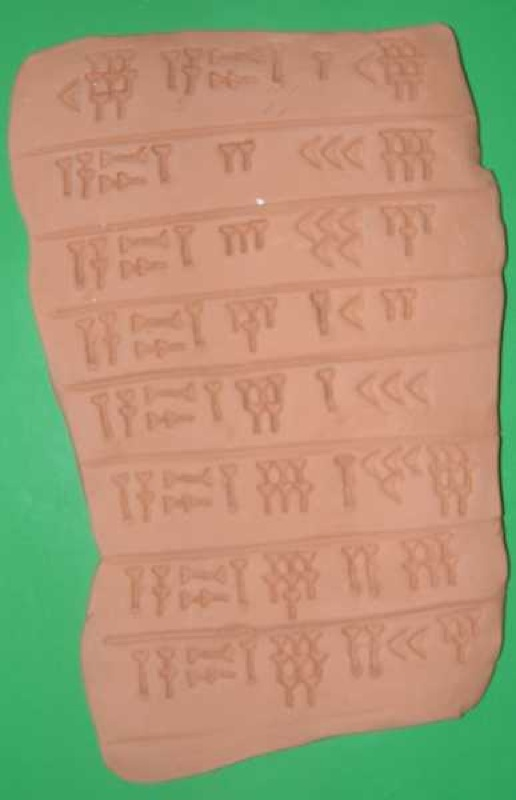
\includegraphics[height=0.3\textwidth]{pictures/babylontafel}\hspace*{0.2cm}
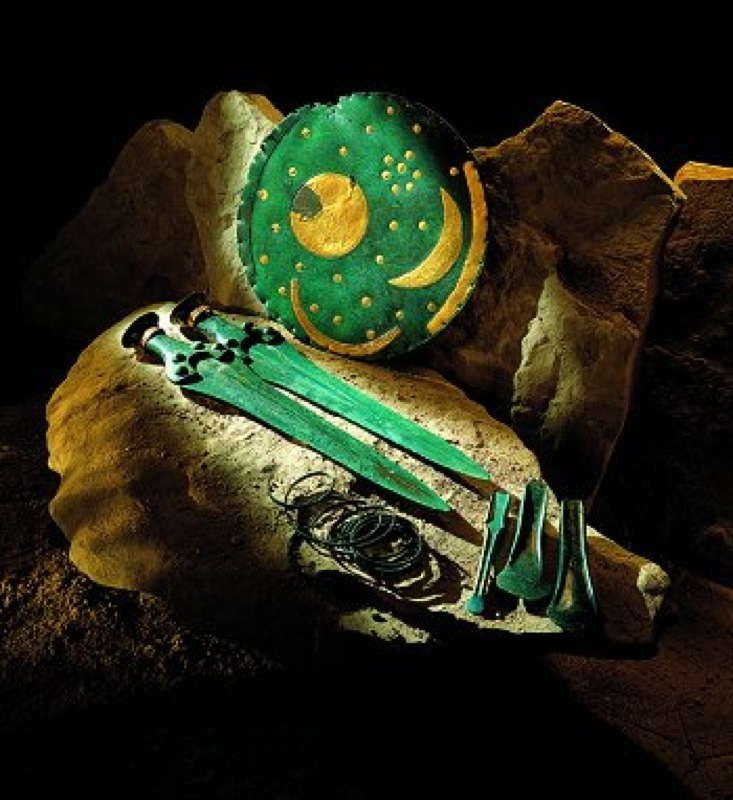
\includegraphics[height=0.3\textwidth]{pictures/babylonuhr}
\end{center}
\caption{Babylonische Rechentafel und Sternkarte}
\end{figure}

Die Babylonier verwendeten als eines der ersten Völker ein \glqq hybrides\grqq{} \definition{Positionssystem}. Der Wert eines Zeichens hängt auch von dessen Position ab. Während wir heute in unserem Dezimalsystem (Basis $10$) die Ziffern $0, 1, 2, \dots, 9$ verwenden, brauchten die Babylonier in ihrem Sechzigersystem $59$ Ziffern; ein Zeichen für die Null, gab es damals noch nicht.

Abschliessend noch ein Beispiel, wie diese Zeichen verwendet werden.
\begin{center}
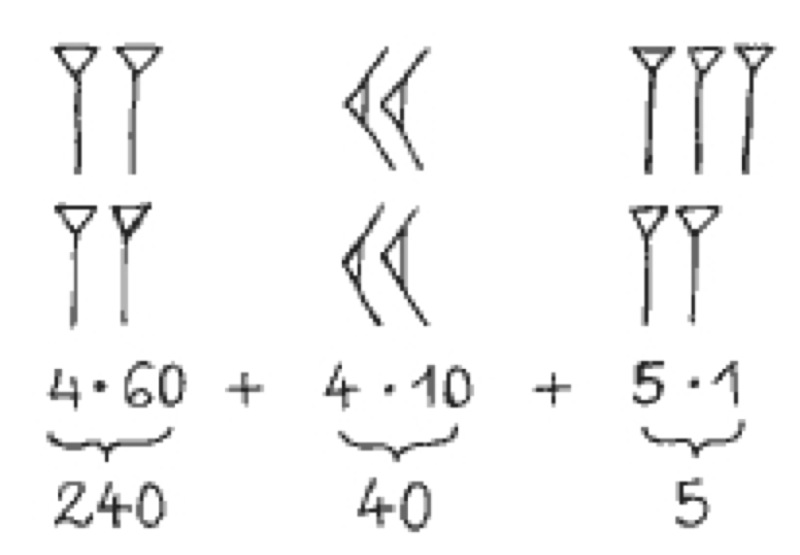
\includegraphics[width=5cm]{pictures/babylon285}
\end{center}

\begin{uebenv}{babylon}
     Welches Zahlensystem verwendeten die Babylonier?
\end{uebenv}



\subsection{Zahlensysteme}

Man unterscheidet im Wesentlichen zwischen Additionssystemen und Positionssystemen.

\subsubsection{Additionssysteme}

In einem Additionssystem wird eine Zahl als Summe der Werte ihrer Ziffern dargestellt. Dabei spielt die Position der einzelnen Ziffern keine Rolle.

\subsubsection{Positionssysteme}

In einem Positionssystem bestimmt die Stelle (Position) den Wert der jeweiligen Ziffer. Die \glqq niederwertigste\grqq\ Position steht dabei ganz rechts.

Ein Stellenwertsystem hat eine Basis $b$. Jede Zifferposition hat einen Wert, der einer Potenz der Basis entspricht. Für die $k$-te Position hat man einen Wert von $b^{k-1}$.

Die Berechnung des Zahlenwertes $z_nz_{n-1}\dots z_0$ erfolgt durch Multiplikation der einzelnen Ziffern $z_i$ mit den zugehörigen Stellenwerten $b_i$ und Addition dieser Produkte:
$$\text{Zahlenwert} = z_n\cdot b^n+\dots+z_i\cdot b^i+\dots+z_0\cdot b^0.$$

\begin{bsp}
Unter der Zahl $1257$ im üblichen Dezimalsystem (d.h. zur Basis $10$) verstehen wir den Wert
$$1\cdot10^3+2\cdot10^2+5\cdot10^1+7\cdot10^0 = 1257.$$
\end{bsp}

Mit der Beschränkung des niedrigsten Exponenten auf $0$ kann man nur ganze Zahlen darstellen. Lässt man auch negative Exponenten zu,
\marginnote{
\qrcode{
https://www.youtube.com/watch?v=bX32IRfefkk}
}
kann man auch rationale Zahlen in einem Stellenwertsystem schreiben. Dabei wird der Übergang vom nichtnegativen zum negativen Exponenten durch ein Trennzeichen markiert, beispielsweise einem Punkt:
$$1\cdot10^2+2\cdot10^1+1\cdot10^0+4\cdot10^{-1}+7\cdot10^{-2}=121.47$$

\begin{uebenv}{binrbiszwanzig}
Die Idee des Positionssystems mit einer bestimmten Basis wird auch beim Binärsystem
\marginnote{
\qrcode{
https://www.youtube.com/watch?v=y96o8U_grVE}
}
(Basis $2$) verwendet.

Die binäre Zahl $1011$ entspricht der Dezimalzahl
$$1\cdot2^3+0\cdot2^2+1\cdot2^1+1\cdot2^0=8+2+1=11.$$
Stelle die Dezimalzahlen von $1$ bis $20$ im Binärsystem dar. Beschreibe dein Vorgehen.
\end{uebenv}



\begin{uebenv}{binzudec}
Verwandle folgende Binärzahlen in Dezimalzahlen
$$1\quad\quad11\quad\quad111\quad\quad1111\quad\quad\dots$$
und
$$10\quad\quad100\quad\quad1000\quad\quad10000\quad\quad\dots$$
\end{uebenv}



\begin{uebenv}{deczubin}
Finde für die Dezimalzahl $34$ die Binärschreibweise.
\end{uebenv}



\subsection{Das Binärsystem}

\subsubsection{Einleitung}

Wie könnte eine Codierung von Zeichen im Computer realisiert werden? Der Computer arbeitet mit elektrischem Strom. Das heisst er kann lediglich die beiden Zustände \glqq Strom an\grqq\ und \glqq Strom aus\grqq\ unterscheiden. Man codiert $1$ für den ersten und $0$ für den zweiten Zustand. Die Information, die durch den Strom in einer Leitung codiert ist, heisst \definition{ein Bit} (binary digit). So lassen sich bloss zwei Zeichen codieren. Kombiniert man aber zwei Leitungen, lassen sich nun vier Zustände unterscheiden:

\begin{center}
\begin{tabular}{c|c}
Leitung 1 & Leitung 2\\ \hline
0 & 0\\
0 & 1\\
1 & 0\\
1 & 1\\
\end{tabular}
\end{center}

\begin{uebenv}{dreileitungen}
Stelle eine Tabelle für drei Leitungen auf.
\end{uebenv}



\begin{uebenv}{minleitungen}
    Wie viele Leitungen braucht man, um alle Buchstaben des Alphabets codieren zu können?
\end{uebenv}



In der Informatik ist es üblich, acht Leitungen zur Speicherung von Informationen zusammenzufassen. Insgesamt lassen sich damit $2^8=256$ verschiedene Zeichen darstellen. Man spricht bei dieser Bündelung von acht Leitungen vom Informationsgehalt ein \definition{Byte}.

\begin{bem}
Früher rechnete man noch in Kilobyte, was ca. 1000 Bytes entspricht. Kilo wurde in diesem Zusammenhang nicht wie üblich für den Wert Tausend verwendet, sondern für $2^{10}=1024\approx1000$. Deshalb ist zum Beispiel ein Megabyte = 1024 Kilobyte.
\end{bem}

Wie rechnet der Computer mit diesen Binärzahlen?

\subsubsection{Rechnen im Binärsystem}

Die Addition von Binärzahlen funktioniert prinzipiell genau so, wie die Addition von Dezimalzahlen.

\begin{uebenv}{binaddieren}
Addiere schriftlich die Binärzahlen $1001011$ und $101011$.
\end{uebenv}



Werden mehrere Binärzahlen addiert, kann der Übertrag natürlich auch grösser als $1$ werden.

\begin{uebenv}{binaddaddieren}
Addiere schriftlich die Binärzahlen $1001011$, $101011$ und $101010$.
\end{uebenv}



\subsubsection{Negative Zahlen}

Schauen wir vierstellige Binärzahlen, sogenannte \definition{Nibbles}, an. Insgesamt können mit einem Nibble $16$ verschiedene Zahlen dargestellt werden. Was passiert nun bei fortlaufender Addition von $1$ ausgehend von der Zahl $0$?
$$0\overset{+1}{\longrightarrow}1\overset{+1}{\longrightarrow}2\overset{+1}{\longrightarrow}\dots\overset{+1}{\longrightarrow}14\overset{+1}{\longrightarrow}15\overset{+1}{\longrightarrow}???$$
Wir können diese Additionskette als Zyklus auffassen, wenn wir die binäre Vierstelligkeit nicht verlassen wollen. Addieren wir nun zur Zahl $1111_{(2)}$ die $1$, so erhalten wir $(1)0000_{(2)}$, also die Zahl $0$ mit einem Überlauf. Wenn Addieren gleichzusetzen mit um eins im Uhrzeigersinn verschieben ist, dann sollte man Subtrahieren mit der Umkehrung definieren.

\begin{uebenv}{nibbles}
Welche Binärzahl repräsentiert  $-7_{(10)}$? Addiere $-7_{(10)}+7_{(10)}$.
\end{uebenv}



Die Frage, die bleibt, ist: Welcher Zahl entspricht die $1000_{(2)}$? Es könnte $-8$ oder $+8$ bedeuten. Man löst dieses Dilemma, indem man einfach ein Vorzeichenbit einführt. Somit können wir also mit einem Nibble die Zahlen $-8$ bis $7$ darstellen.

Genau diesen Zusammenhang kann man zur Berechnung der Darstellung einer negativen Zahl im Binärsystem verwenden:
\begin{itemize}
\item Ist eine Zahl gegeben, so bildet man zuerst das sogenannte Einerkomplement, indem man einfach jedes der $8$ Bit \glqq kippt\grqq.
\item Danach addiert man noch $1$ zum Einerkomplement.
\end{itemize}

\begin{bsp}
Wir betrachten die Zahl $23=00010111_{(2)}$. Durch Kippen erhält man $11101000$. $1$ addieren bringt $11101001=-23$.
\end{bsp}

Wir sind nun in der Lage, die Subtraktion im Binärsystem zu lösen, indem wir sie auf die Addition zurückführen.
\begin{align*}
127-19&=127+(-19)\\
&=0111\,1111_{(2)} + 1110\,1101_{(2)}\\
&=(1)0110\,1100_{(2)}\\
&=108
\end{align*}

\begin{uebenv}{negativebin}
Prüfe durch Rechnung obiges Beispiel. Berechne danach im Binärsystem

\begin{enumerate}[a)]
\item $115-48$
\item $77-76$
\end{enumerate}
\end{uebenv}




\subsubsection{Multiplikation}

Neben der Addition und Subtraktion von Binärzahlen spielt die Multiplikation von Binärzahlen eine wesentliche Rolle. Wir kennen ein Verfahren in den Dezimalzahlen, welches wir direkt auf das Binärsystem anwenden können. Jedoch liegt dabei der Schwerpunkt auf dem Addieren, wie das folgende Beispiel zeigt.

\begin{bsp}
Wir berechnen das Produkt von $0000\,1001_{(2)}$ und $0010\,0111_{(2)}$. Dezimal erhalten wir $9\cdot23=207$. Binär

\begin{uebenv}{binprod}
Berechne $9\cdot23$ binär.
\end{uebenv}


\end{bsp}

Bei der Multiplikation entstehen so bis zu acht Summanden, die anschliessend addiert werden müssen, dagegen ist die Multiplikation als solches sehr einfach. Ferner sieht man nun im Ergebnis zwei Bytes aneinander gereiht. Dabei haben wir Glück und das zweite Byte bleibt mit Nullen gefüllt, so dass unser Resultat wieder in ein Byte hinein passt. Es könnte ja auch sein, dass das vordere Byte benötigt wird, nämlich dann, wenn das Ergebnis grösser als $255$ ist.

\begin{uebenv}{binhex}
Vergleiche das Binärsystem mit dem Hexadezimalsystem. Beschreibe, wie man ohne grossen Rechenaufwand Zahlen im Hexadezimalsystem ins Binärsystem umwandeln kann.
\end{uebenv}



\clearpage

\subsection{Notizen zu den Übungen}

\begin{lsg}{dezimal}
     Wir Schweizer rechnen im Dezimalsystem, $10$-er System. Wie der Name sagt, brauchen wir in diesem Positionssystem $10$ Ziffern: $0$, $1$, $2$, \dots , $9$.
\end{lsg}
\begin{lsg}{babylon}
    Die Babylonier verwendeten das $60$-er System, auch Sexagesimalsystem genannt. Überbleibsel davon stecken beispielsweise in der Zeit- (Minuten, Sekunden) oder Winkelmessung (Grad, Minuten, Sekunden).
\end{lsg}
\begin{lsg}{binrbiszwanzig}
\begin{tabular}{|c|c|c|c|}
  \hline
  \textbf{BIN} & \textbf{DEC} & \textbf{BIN} & \textbf{DEC} \\
  \hline
  0001 & 1 & 1011 & 11 \\
  0010 & 2 & 1100 & 12 \\
  0011 & 3 & 1101 & 13 \\
  0100 & 4 & 1110 & 14 \\
  0101 & 5 & 1111 & 15 \\
  0110 & 6 & 10000 & 16 \\
  0111 & 7 & 10001 & 17 \\
  1000 & 8 & 10010 & 18 \\
  1001 & 9 & 10011 & 19 \\
  1010 & 10 & 10100 & 20 \\
  \hline
\end{tabular}
\end{lsg}
\begin{lsg}{binzudec}
\begin{enumerate}[a)]
    \item $1$, $3$, $7$, $15$, $2^{k}-1$
    \item $2$, $4$, $8$, $16$, $2^k$
\end{enumerate}
\end{lsg}
\begin{lsg}{deczubin}
Ich gucke, welche Zweierpotenz noch Platz hat und fahre dann mit dem Rest analog fort. Man kann auch stetig durch zwei Teilen und am Ende die Binärzahl rückwärts zusammensetzen.
\begin{enumerate}[a)]
    \item $34=2^5+2^1=100010_{(2)}$
    \item $34\div2\equiv0$, $17\div2\equiv1$, $8\div2\equiv0$, $4\div2\equiv0$, $2\div2\equiv0$, $1\div2\equiv1$. Wenn man die Reste nun rückwärts auflistet, hat man die Zweierpotenzen-Aufspaltung von $34$, also $34=100010_{(2)}$.
\end{enumerate}
\end{lsg}
\begin{lsg}{dreileitungen}
\begin{center}
\begin{tabular}{c|c|c}
Leitung 1 & Leitung 2 & Leitung 3\\ \hline
0 & 0 & 0\\
0 & 0 & 1\\
0 & 1 & 0\\
0 & 1 & 1\\
1 & 0 & 0\\
1 & 0 & 1\\
1 & 1 & 0\\
1 & 1 & 1
\end{tabular}
\end{center}
\end{lsg}
\begin{lsg}{minleitungen}
    Für das Alphabet mit 26 Buchstaben braucht man mindestens $5$ Leitungen, da $2^4=16$ und $2^5=32$. Als Standardgrösse hat sich ein \definition{Byte}, $2^8=256$ Zustände, etabliert.
\end{lsg}
\begin{lsg}{binaddieren}
    \begin{align*}
        1001001 &\\
        +\phantom{01}101011 &\\
        \hline
        1110100&
    \end{align*}
\end{lsg}
\begin{lsg}{binaddaddieren}
\begin{align*}
    1001011 &\\
    +\phantom{01}101011 &\\
    +\phantom{01}101010 &\\
    \hline
    10100000
\end{align*}
\end{lsg}
\begin{lsg}{nibbles}
$-7=1001_{(2)}$ und $7=0111_{(2)}$.

\begin{align*}
    \phantom{0}1001 &\\
    +\phantom{0}0111 &\\
    \hline
    (1)0000
\end{align*}
\end{lsg}
\begin{lsg}{negativebin}
\begin{enumerate}[a)]
\item $01110011-00110000=01110011+11010000=(1)01000011$
\item $77-76 01001101-01001100=01001101+10110100=(1)00000001$
\end{enumerate}
\end{lsg}
\begin{lsg}{binprod}
    \centering
    \begin{tabular}{c c c c c c c c c c c c c c c c c}
        0 & 0 & 0 & 0 & 1 & 0 & 0 & 1 & $\cdot$ & 0 & 0 & 0 & 1 & 0 & 1 & 1 & 1\\
         & & & & & & & & & 0 & 0 & 0 & 1 & 0 & 1 & 1 & 1\\
         & & & & & & 0 & 0 & 0 & 1 & 0 & 1 & 1 & 1 & 0 & 0 & 0\\
         \hline
         &&&&&&&&&1&1&0&0&1&1&1&1
    \end{tabular}
\end{lsg}
\begin{lsg}{binhex}
Es ist $2^4=16$ und daher kann man immer einen Viererblock binär als Hexadezimalzahl notieren. Zum Beispiel ist $1\,0010_{(2)}=12_{(16)}$ oder $A2_{(16)}=1010\,0011$.
\end{lsg}

\clearpage

\section{Modulo}
Modulare Arithmetik --- rechnen mit Resten --- ist ein nützliches Werkzeug der Zahlentheorie.
\begin{figure}
  \begin{center}
    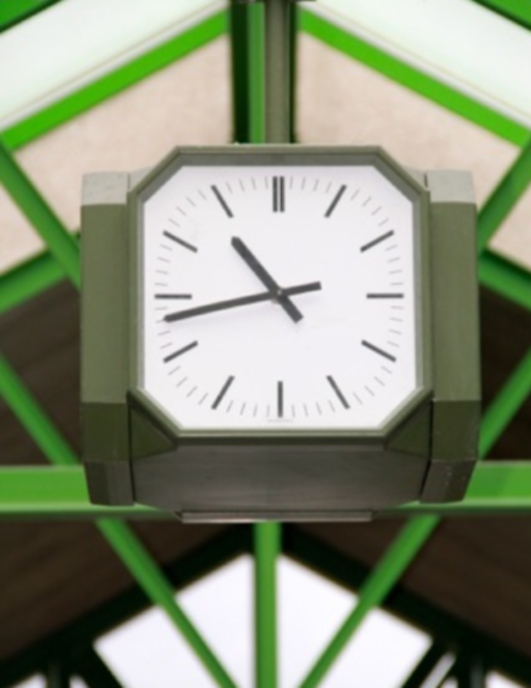
\includegraphics[width=0.3\textwidth]{pictures/uhr}
  \end{center}
%\caption{A gull}
\end{figure}

\subsection{Ein erstes Beispiel}

Wir wissen, dass die Menge $\mathbb{Z}$ in zwei Klassen aufgespalten werden kann.

\begin{itemize}
\item die geraden Zahlen:
$$\dots,-6,-4,-2,0,2,4,6,\dots$$
\item die ungeraden Zahlen:
$$\dots,-5,-3,-1,1,3,5,\dots$$
\end{itemize}

Nun können wir gewisse Verallgemeinerungen über die Gesetzmässigkeiten dieser Zahlen formulieren; in Abhängigkeit ihrer Zugehörigkeit zu einer der beiden Klassen. Beispielsweise ist die Summe zweier gerader Zahlen wieder gerade. Die Summe einer geraden und einer ungeraden Zahl ist ungerade. Die Summe zweier ungeraden Zahlen ist gerade. Das Produkt zweier gerader Zahlen ist gerade, usw.

\subsection{Motivation}

Im obigen Beispiel ist der sogenannte \definition{Modulus} gleich $2$. Der Modulus kann als Anzahl der Klassen betrachtet werden, in die unsere Zahlenmenge $\mathbb{Z}$ aufgeteilt wird.

Jetzt legen wir für jede der beiden Klassen ein Symbol fest. Wir schreiben $0$ für die Klasse aller geraden Zahlen und $1$ für die Klasse aller ungeraden Zahlen\footnote{Präziser müsste man zum Beispiel $\overline{0}$ für die Klasse der geraden Zahlen schreiben, weil $0$ selber ja ein Element der Klasse der geraden Zahlen ist.}. Die Bezeichnung erfolgte willkürlich; wir hätten auch $2$ und $1$, oder $-32$ und $177$ wählen können. $0$ und $1$ sind aber die üblichen Bezeichnungen.

Die Aussage

\begin{quote}
Die Summe zweier gerader Zahlen ist eine gerade Zahl.
\end{quote}

wird wie folgt schlank geschrieben:

$$0+0\equiv0\mod 2$$

Hier bezeichnet das Symbol $\equiv$ nicht Gleichheit, sondern \definition{Kongruenz}. $\mod 2$ bedeutet, dass unser Modulus $2$ ist. Obige Aussage liest man: \glqq Null plus Null ist kongruent Null Modulo Zwei\grqq. Die Aussage, dass die Summe einer geraden und einer ungeraden Zahl ungerade ist, schreibt sich
$$0+1\equiv1\mod2.$$

Diese Beispiele sind trivial. Wie aber schreiben wir, dass die Summe zweier ungerader Zahlen gerade ist?
$$1+1\equiv0\mod2.$$

Analoge Aussagen erhält man für die Multiplikation:
\begin{align}
0\cdot0\equiv0\mod2\notag\\
0\cdot1\equiv0\mod2\notag\\
1\cdot1\equiv1\mod2\notag
\end{align}

\subsection{Definition und weitere Beispiele}

Selbverständlich kann man auch Modulo $m$, $m\in\mathbb{N}$, rechnen. Wir definieren

\begin{cdef}[Modulo]
Sei $m\in\mathbb{N}$. Zwei Zahlen $a,b\in\mathbb{Z}$ heissen kongruent Modulo $m$, falls ein $k\in\mathbb{Z}$ existiert, so dass $a-b=k\cdot m$. Man schreibt
$$a\equiv b\mod m.$$
\end{cdef}

\begin{bsp}
$5$ und $8$ sind kongruent Modulo $3$, denn es gilt $5-8=-1\cdot 3$.
\end{bsp}

Wir betrachten ganze Zahlen Modulo $3$. Klar ist, dass alle Vielfachen von $3$, $3n$, kongruent Modulo $3$ sind, da jede Differenz zweier solcher Zahlen durch $3$ teilbar ist. Analog sind alle Zahlen der Form $3n+1$ und alle Zahlen der Form $3n+2$ kongruent Modulo $3$, $n\in\mathbb{Z}$.

\begin{align}
\dots\equiv-6\equiv-3\equiv0\equiv3\equiv6\equiv9\dots\mod3\notag\\
\dots\equiv-7\equiv-4\equiv-1\equiv2\equiv5\equiv8\dots\mod3\notag\\
\dots\equiv-8\equiv-5\equiv-2\equiv1\equiv4\equiv7\dots\mod3\notag
\end{align}

\subsection{Die Uhr}

Ein alltäglicher Fall ist der Modulus $12$. Man nennt den Fall $m=12$ auch die \glqq Uhr-Arithmetik\grqq.

\begin{bsp}
Wenn es 07:00 Uhr ist, welche Zeit haben wir in $\unit[25]{Stunden}$. Da $25\equiv1\mod12$ können wir einfach $1$ zu $7$ addieren:
$$7+25\equiv7+1\equiv8\mod12.$$
Also 08:00 Uhr.
Die Sekunden und Minuten auf der Uhr sind auch modular, nämlich Modulo $60$.
\end{bsp}

\subsection{Rechenregeln}

Die Grundlage für folgende Rechenregeln ($a,b\in\mathbb{Z}$ und $m,n\in\mathbb{N}$) mit Moduln bildet

\begin{csatz}[Modulare Aequivalenz]
$$
a\equiv b\mod m \quad\Leftrightarrow\phantom{:}\quad a-b\equiv 0\mod m\Leftrightarrow:\quad m\mid(a-b)
$$
\end{csatz}

Die restlichen Sätze, inklusive die Äqui\-valenz\-eigen\-schaf\-ten, folgen unmittelbar.

\begin{csatz}[Additon mod]
$$a\equiv b\mod m \quad\Rightarrow\quad a+c\equiv b+c\mod m$$
\end{csatz}

\begin{csatz}[Multiplikation mod]
$$a\equiv b\mod m \quad\Rightarrow\quad ac\equiv bc\mod m$$
\end{csatz}

\begin{csatz}[Potenz mod]
$$a\equiv b\mod m \quad\Rightarrow\quad a^n\equiv b^n\mod m$$
\end{csatz}

\begin{csatz}[Additivität mod]
$$
a\equiv b\mod m \text{ und } c\equiv d\mod m\quad\Rightarrow\quad a+c\equiv b+d\mod m
$$
\end{csatz}

\begin{csatz}[Multiplikativität mod]
$$
a\equiv b\mod m \text{ und } c\equiv d\mod m\quad\Rightarrow\quad ac\equiv bd\mod m
$$
\end{csatz}

\begin{csatz}[Chinese mod]
$$
\gcd(m,n)=1, a\equiv b\mod m \text{ und } a\equiv b\mod n\quad\Rightarrow\quad a\equiv b\mod mn
$$
\end{csatz}

\begin{csatz}[Primzahlprodukt]
Ist $p$ eine Primzahl, so gilt
$$
ab\equiv 0\mod p\quad\Rightarrow\quad a\equiv 0\mod p\textup{ oder }b\equiv0\mod p
$$
\end{csatz}

\begin{proof}
    Sei $p$ prim und $ab\equiv0\mod p$. $\exists k\in\mathbb{Z}$ mit $ab-0=ab=kp$, also teilt $p$ das Produkt $ab$. Wegen der Eindeutigkeit der Primfaktorzerlegung muss $p$ entweder in der Zerlegung von $a$ oder von $b$ vorkommen. Das heisst $p|a$ oder $p|b$.
\end{proof}

\begin{csatz}[Kürzungssatz]
$$
\gcd(a,m)=1 \textup{ und } ab\equiv ac\mod m\quad\Rightarrow\quad b\equiv c\mod m
$$
\end{csatz}

\begin{proof}
    Sei $\gcd(a,m)=1$ und $ab\equiv ac\mod{m}$. Es folgt $ab-ac=a(b-c)\equiv0\mod{m}$. Da $\gcd(a,m)=1$ folgt $m|(b-c)$ und nach Definition $b\equiv c\mod{m}$.
\end{proof}

\begin{uebenv}{modulostze}
Gib konkrete Beispiele zu den Sätzen und beweise sie.
\end{uebenv}




\subsection{Eigenschaften der Kongruenz}

Man zeigt einfach, dass für beliebige $a,b,c$ und $m\neq0$ folgende Eigenschaften erfüllt sind:

\begin{itemize}
\item $a\equiv a\mod m$ (Reflexivität)
\item Falls $a\equiv b\mod m$, dann gilt $b\equiv a\mod m$ (Symmetrie)
\item Falls $a\equiv b\mod m$ und $b\equiv c\mod m$, dann $a\equiv c\mod m$ (Transitivität)
\end{itemize}

\begin{cdef}[Äquivalenzrelation]
Eine Relation, die obige drei Bedingungen erfüllt, nennt man Äquivalenzrelation. Die Äquivalenzrelation $\mod m$ teilt $\mathbb{Z}$ in $m$ \definition{Äquivalenzklassen}.
\end{cdef}

Man schreibt manchmal für die Äquivalenzklasse
\marginnote{
\qrcode{
https://www.youtube.com/watch?v=USC0Nm413FE}
}
einer Zahl $a$ etwa $[a]$ oder auch $\overline{a}$, um zwischen Zahl und Klasse zu unterscheiden.

\begin{figure}
\begin{center}
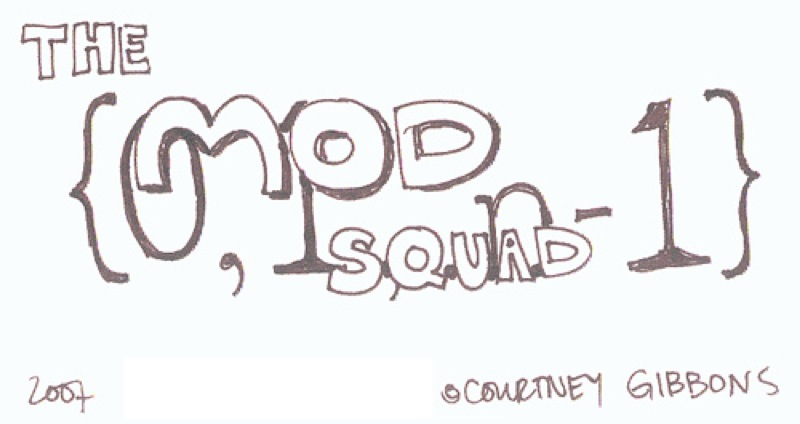
\includegraphics[width=0.618\textwidth]{pictures/modsquad}
\end{center}
\caption{The Mod Squad}
\end{figure}

\begin{uebenv}{glsysmod}
Zeige, dass das Gleichungssystem
\begin{align}
11x-5y=7\\
9x+10y=-3
\end{align}
keine ganzzahlige Lösung besitzt.
\end{uebenv}



\begin{uebenv}{pythagoras}
Zeige, dass für $x,y,z\in\mathbb{Z}$ mit
$$x^2+y^2=z^2$$
mindestens eine der Zahlen durch $2$, mindestens eine durch $3$ und mindestens eine durch $5$ teilbar ist.
\end{uebenv}



\clearpage

\section{Teilbarkeit}
\subsection{Teilbarkeit durch 3}

Es gilt
\begin{csatz}[Teilbarkeit durch 3]
Eine
\marginnote{
\qrcode{
https://youtu.be/Vo63939DIa8}
}
Zahl ist genau dann durch $3$ teilbar, wenn es ihre Quersumme ist.
\end{csatz}

\begin{proof}
Sei $n\in\mathbb{N}$ im Dezimalsystem als
$$n=a_ra_{r-1}\dots a_1a_0$$
geschrieben, so ist explizit
$$n=a_0+10\cdot a_1+\dots+10^r\cdot a_r.$$
Modulo $3$ ist jetzt $10\equiv1\mod3$, also $[10]=[1]$. Damit ist
\begin{align*}
[n]&=[a_0+10\cdot a_1+\dots+10^r\cdot a_r]\\
&=[a_0]+[10]\cdot[a_1]+\dots+[10]^r\cdot[a_r]\\
&=[a_0]+[a_1]+\dots+[a_r]\\
&=[a_0+a_1+\dots+a_r]
\end{align*}
das heisst, die Zahl $n$ ist Modulo $3$ gleich ihrer Quersumme. Insbesondere ist $n$ genau dann durch $3$ teilbar, wenn die Quersumme dies ist.
\end{proof}

\begin{figure}
\begin{center}
    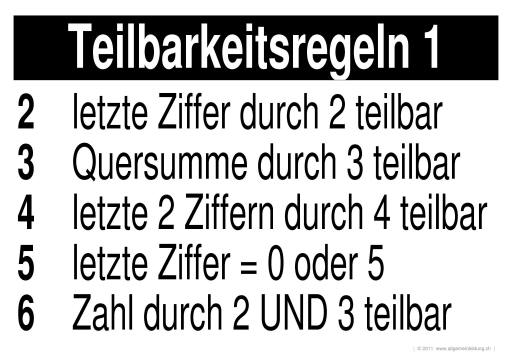
\includegraphics[width=0.382\textwidth]{pictures/regeln}
  \end{center}
%\caption{Teilbarkeit}
\end{figure}

\begin{uebenv}{teilbarkeitdurchelf}
    Vervollständigen und begründen Sie folgende Aussage:
    \begin{quote}
        Eine natürliche Zahl ist genau dann durch \dots teilbar, wenn es ihre alternierende Quersumme ist.

        Unter der \emph{alternierenden Quersumme} verstehen wir die von rechts nach links gelesene \glqq Quersumme\grqq{} mit abwechselnden Vorzeichen. Also beispielsweise wäre zur Zahl $123$ die alternierende Quersumme $3-2+1=2$.
    \end{quote}
\end{uebenv}



\subsection{Teilbarkeit durch 11}

Mit der Überlegung aus dem vorigen Beispiel lässt sich rasch eine Bedingung für die Teilbarkeit einer Zahl durch $11$ herleiten. Es ist $10\equiv-1\mod11$, also ist analog zur obigen Rechnung für eine Dezimalzahl
$$n\equiv a_0-a_1+a_2-\dots+(-1)^ra_r\mod11.$$
Auf der rechten Seite steht hier die alternierende Quersumme. Eine Zahl ist also genau dann durch $11$ teilbar, wenn es ihre alternierende Quersumme ist.

\begin{bsp}
$12375$ ist durch $11$ teilbar, denn
$$5-7+3-2+1=0.$$
\end{bsp}

\subsection{Teilbarkeit im Hexadezimalsystem}

\begin{uebenv}{hexateilbarkeit}
Überlege dir Teilbarkeitsregeln im Hexadezimalsystem. Betrachte dazu die Teilbarkeit einer Hexadezimalzahl durch $3$, $5$ und $17$.
\end{uebenv}



\clearpage

\subsection{Notizen zu den Übungen}

\begin{lsg}{modulostze}
Zum Beispiel zur Addition:

$$4\equiv10\mod3\Leftrightarrow 4+2\equiv10+2\mod3.$$

\begin{proof}
Beweis über die Definition: Gelte $a\equiv b\mod n$ und sei $c\in\mathbb{Z}$ beliebig. Das heisst $\exists k\in\mathbb{Z}$ mit $b-a=kn$ und daraus
$$kn=b-a=(b+c)-(a+c).$$
Das heisst $a+c\equiv b+c\mod{n}$.
\end{proof}

Die übrigen Sätze zeigt man analog oder verwendet bereits bewiesene.
\end{lsg}
\begin{lsg}{glsysmod}
Modulo $2$ gilt:
\begin{align}
x+y\equiv1\\
x\equiv1
\end{align}
Also ist $x$ ungerade und $y$ gerade.
Modulo $5$ gilt:
\begin{align}
x\equiv2\\
4x\equiv2
\end{align}
Es folgt $5x\equiv4$, Widerspruch, da $5x\equiv0\mod5$!
\end{lsg}
\begin{lsg}{pythagoras}
Modulo $2$ betrachten wir die Fälle $z^2\equiv0$ und $z^2\equiv1$. Im ersten Fall gälte dann $x^2\equiv0$ und $y^2\equiv0$ oder $x^2\equiv1$ und $y^2\equiv1$. Für den zweiten Fall gilt oEdA $x^2\equiv1$ woraus $y^2\equiv0$ und damit $y\equiv0$ folgt. Also ist immer sicher mindestens eine Zahl durch $2$ teilbar.

Modulo $3$ gelte $z^2\equiv1$. Dann muss oEdA $x^2\equiv1$ und $y^2\equiv0$ gelten, also $y\equiv0\mod{3}$. Oder es wäre $x^2\equiv2$ und $y^2\equiv2$. Aber das kann wegen $x\equiv\sqrt{2}$ nicht passieren.
Aus dem gleichen Grund muss $z^2\equiv2$ nicht betrachtet werden und für $z^2\equiv0$ ist die Behauptung trivial. Somit ist mindestens eine Zahl durch $3$ teilbar.

Modulo $5$ äquivalent zu $0$ ist wiederum trivial. Gelte noch Modulo $5$ $z^2\equiv1$ oder $z^2\equiv4$. Im ersten Fall sind nur möglich $x\equiv1$ und $y\equiv0$ oder viceversa. Im zweiten Fall klappt nur $x\equiv4$ woraus $y\equiv0$ folgt. Also ist sicher mindestens eine Zahl durch $5$ teilbar.
\end{lsg}
\begin{lsg}{teilbarkeitdurchelf}
\begin{proof}
    Die Antwort ist $11$. Denn für $n\in\mathbb{N}_0$ gilt
    $$10^n\equiv(-1)^n\mod11,$$
da ja $10\equiv -1\mod11$.
Daraus folgt
\begin{align*}
    & a_k\cdot10^k+a_{k-1}\cdot10^{k-1}+\dots+ a_1\cdot10^1+a_0\cdot10^0\\
        &\equiv a_k\cdot(-1)^k+a_{k-1}\cdot(-1)^{k-1}+\dots+ a_1\cdot(-1)^1+a_0\cdot(-1)^0\mod11\\
        &\equiv (-1)^k a_k+(-1)^{k-1}a_{k-1}+\dots- a_1+a_0\mod11
\end{align*}
Das heisst man kann bequem von rechts nach links die alternierende Quersumme bilden und gucken, ob die durch $11$ teilbar ist.
\end{proof}
\end{lsg}
\begin{lsg}{hexateilbarkeit}
        Für das Hexadezimalsystem ($16$er System) könnte man eine Teilbarkeitsregel mit Quersumme für die Teilbarkeit mit $3$ oder $5$ formulieren, da für $n\in\mathbb{N}_0$ gilt: $16^n\equiv 1\mod3$ bzw. $\mod5$. Für die alternierende Quersumme kann man sinngemäss eine Teilbarkeitsregel $\mod17$ formulieren, da $16^n\equiv(-1)^n\mod17$.
\end{lsg}

\clearpage

\section{Barcode}
Ein ähnliches System und Prüfverfahren existiert für die wohlbekannten Barcodes zum Beispiel auf Verpackungen.

\begin{figure}
\begin{center}
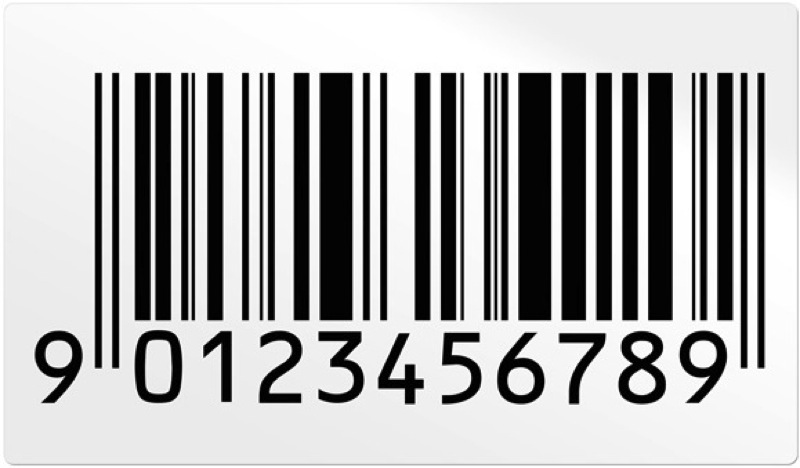
\includegraphics[width=0.5\textwidth]{pictures/barcode}
\end{center}
\caption{Barcode EAN 13}
\end{figure}

Bezahlt man in einem Geschäft seine Ware, so wird der Preis in aller Regel nicht per Hand eingegeben. Vielmehr wird der Strichcode, der sich auf jedem Artikel befindet, eingescannt; und selbst wenn dies aufgrund technischer Probleme nicht funktioniert, gibt der Kassierer nicht den Preis, sondern die zum Strichcode gehörende Ziffernfolge ein. Wie kommt es, dass ein Fehler beim Eingeben immer auffällt?

Man braucht also eine Idee, wie man Fehler bei der Eingabe mit hoher Wahrscheinlichkeit bemerken kann; und die Idee heisst Redundanz. Man hängt an den Teil des Codes, den man zur Identifikation des Produkts braucht, zusätzliche (redundante) Ziffern an, deren einziger Sinn es ist, den Code fehlerresistenter zu machen. Dabei sollten möglichst wenig zusätzliche Ziffern eine möglichst hohe Sicherheit bieten. Weshalb und wie man das mit nur einer Ziffer erreichen kann hat mit Modulo Arithmetik und Gruppen zu tun. Ähnliche Verfahren werden auch bei Kreditkarten, ISBN-Nummern, Seriennummer von Geldscheinen etc. verwendet.

\clearpage

\section{Die alte ISBN-Nummer}
\subsection{Prüfziffern}

Als ein kleines Beispiel beschreiben wir das alte ISBN-System. Dieses ist zwar nicht mehr ganz aktuell, aber für unsere Zwecke instruktiver als die inzwischen verwendete Variante.

Jedem Buch ist eine zehnstellige ISBN-Nummer zugeordnet, die zur eindeutigen Identifikation dient. Von diesen $10$ Ziffern sind die ersten $9$ die eigentliche Information, die zehnte ist eine Prüfziffer. Diese soll eine gewisse Sicherheit zur Vermeidung von Tipp- und Übertragungsfehlern gewährleisten.
Bezeichne
$$Y=a_1a_2a_3\dots a_9a_{10}$$
eine ISBN Nummer. Dabei ist $a_i\in\{0,1,2,\dots,9\}$ und
$$a_{10}\equiv a_1+2a_2+3a_3+\dots+9a_9=\sum_{i=1}^9ia_i\mod11.$$
Dies ergibt einen Wert zwischen $0$ und $10$. Falls man $10$ erhält schreibt man ein X.

\begin{bsp}
Wir nehmen als Beispiel das Buch
\begin{quote}
P.~Hartmann, \emph{Mathematik für Informatiker}, Vieweg, 2003.
\end{quote}
mit der (alten) ISBN-Nummer 3--8348--0096--1.
\end{bsp}

Natürlich kann man nicht erwarten, dass so alle Fehler erkannt werden. Aber, wie wir gleich sehen werden, schützt das Modul $11$ vor den alltäglichen.

\subsection{Ziffer fehlerhaft eingetippt}

Geschieht der Fehler in der Prüfziffer selbst, dann ist der Fall klar. Wir können also den Fehler zwischen $1$ und $9$ annehmen und müssen zeigen, dass die Prüfziffer falsch ist. Sei also
$$Y'=a_1\dots a_i'\dots a_{10}$$
die fehlerhafte ISBN mit dem Fehler an der $i$-ten Stelle, $1\leq i\leq9$. Die Prüfziffer wäre so
$$a'_{10}=\sum_{j\neq i}ja_j+ia_i'\mod11$$
Wir haben aber $a_{10}$ und es gilt
$$a_{10}-a_{10}'=ia_i-ia_i'=i(a_i-a_i')\mod11$$
Wegen $a_i\neq a_i'$ ist $a_i-a_i'\neq0$ und wegen $1\leq i\leq9$ auch $i\neq0$. Daraus folgt mit einer nicht ganz trivialen Überlegung, dass $i(a_i-a_i')\not\equiv0\mod11$. Dabei ist die Wahl des Moduls wichtig. Entscheidend für die letzte Folgerung ist, dass $11$ eine Primzahl ist, denn für diese haben wir

\begin{csatz}[Primfaktorsatz]
Sind $p$ prim und $a,b\in\mathbb{Z}$ mit $p|ab$, so gilt $p|a$ oder $p|b$.
\end{csatz}

Wir brauchen die Negation des obigen Satzes: Teilt $p$ weder $a$ noch $b$, dann teilt $p$ auch nicht $ab$.

\begin{proof}
Wenn $p$ weder $a$ noch $b$ teilt, dann kommt $p$ nicht in der Primfaktorzerlegung von $a$ und $b$ vor, also auch nicht in der Primzahlzerlegung des Produkts $ab$. Das heisst $p$ teilt $ab$ nicht.
\end{proof}

Damit ist gezeigt, dass insbesondere für $p=11$ der letzte Schritt gilt und damit die Prüfziffer der ISBN eine fehlerhafte Ziffer erkennt.

\begin{uebenv}{isbn}
    Früher wurde für die Buchklassifikation anstelle der heute gebräuchlichen ISBN13- die \textbf{ISBN10}-Nummer verwendet. Diese beiden Nummern unterscheiden sich nur durch das Präfix $978$ und die Prüfziffer, die restlichen $9$ Ziffern stimmen überein. Ich habe mich in dieses Beispiel für die ISBN10 entschieden, da sie rechnerisch etwas handlicher ist.
    
    Das Buch \emph{Mathematik für Informatiker} hat die ISBN-10 Nummer $3-8348-0096-1$
    
    \begin{center}
        \makebox[0pt]{\EANisbn}
    \end{center}
    
    wobei die letzte Ziffer, $1$, als Prüfziffer (Checksum) fungiert. Diese letzte Ziffer $a_{10}$ wird in der ISBN10-Variante aus den vorangehenden Ziffern wie folgt berechnet:
    $$a_{10}\equiv\sum_{k=1}^9k\cdot a_k\mod11.$$

    \begin{enumerate}[a)]
        \item Überprüfe, ob die Checksum $1$ korrekt ist. 
        \item Wähle eine beliebige Position in der ISBN-Nummer aus und vertippe dich (absichtlich). Berechnen nun die Prüfziffer der \glqq vertippten\grqq{} Nummer.
        \item Angenommen, man vertippe sich an genau $2$ Stellen, sagen wir Positionen $2$ und $5$. Registriert die Prüfziffer die Vertipper? Finde ein Beispiel für einen \glqq Doppelvertipper\grqq, der nicht erkannt wird.
        \item In wieviel Prozent der Fälle registriert die Prüfziffer den Vertipper an diesen Positionen nicht?
    \end{enumerate}
\end{uebenv}



\begin{bem}
All dies würde nicht funktionieren, wenn wir anstelle von $11$ beispielsweise $10$ als Modul verwendet hätten. Denn wegen $10=2\cdot5$, also $2\cdot5\equiv0\mod10$ würde etwa ein Fehler an der $i=5$-ten Stelle nicht erkannt, wenn die fehlerhafte Ziffer um $2$ von der korrekten Ziffer abweicht. Die Prüfziffer Modulo $10$ bliebe unverändert.
\end{bem}

\begin{uebenv}{isbnpython}
    Schreibe eine Python-Funktion, die zu gegebenem Input einer ISBN10-Nummer als Output angibt, ob die Nummer korrekt ist oder nicht.

    Verwende anschliessend das Programm um zu testen, dass die Prüfziffer bemerkt, falls man zwei Ziffern vertauscht hat.
\end{uebenv}



\begin{uebenv}{isbnmodzehn}
    Zeige, dass die Checksum (siehe Aufgabe \ref{exercise:isbn10} auf Seite \pageref{exercise:isbn10}) einen Vertauscher bemerkt. Zeige dies für $2$
 Ziffern, die nicht zwingend aufeinander folgen.
 \end{uebenv}



\begin{uebenv}{isbndreizehn}
    Bei der ISBN13 berechnet sich die Prüfziffer $z_{13}$ via
    $$z_{13}\equiv10-\left(\sum_{k=1}^{12}z_k\cdot 3^{(k+1)\mod2}\mod10\right)\mod10.$$
    Überprüfen Sie die Korrektheit der ISBN13 Prüfziffer aus Aufgabe \ref{exercise:isbn10} auf Seite \pageref{exercise:isbn10}.
\end{uebenv}




\begin{bem}
Wie oben gesehen, ist also die Wahl des Moduls entscheidend. Bei $9$ informationstragenden Ziffern braucht man also eine Primzahl grösser oder gleich $10$, und $11$ ist dafür die kleinstmögliche Wahl.
\end{bem}

\subsection{Zahlendreher}

Die
\marginnote{
\qrcode{
https://youtu.be/2VNHnWVAP_8}
}
ISBN erkennt nicht nur einzelne fehlerhafte Ziffern, sondern auch den am häufigsten auftauchende Fehlertyp: das Vertauschen zweier aufeinanderfolgender Ziffern. In der Tat erkennt die Prüfziffer sogar Vertauschen von nicht unmittelbar aufeinanderfolgenden Ziffern, was zwar weniger vorkommt, aber für den folgenden Beweis ohne Mehraufwand mit einbezogen werden kann.

Sei
$$Y'=a_0\dots a_{i-1}a_ja_{i+1}\dots a_{j-1}a_ia_{j+1}\dots a_{10}$$
eine falsche ISBN, die durch Vertauschen der $i$-ten mit der $j$-ten Ziffer entstand, $1\leq i<j\leq9$. Zwei Fälle lassen wir aussen vor. Erstens, dass die Prüfziffer eine der vertauschten Ziffern ist (diesen Fall könnte man separat behandeln), und zweitens, dass die vertauschten Ziffern identisch sind, dann hätte ja der Verdreher keine Wirkung. Als Prüfziffer für $Y'$ erhält man so
$$a_{10}'\equiv\sum_{k\neq i,j}ka_k+ia_j+ja_i\mod11,$$
also
\begin{align*}
a_{10}-a_{10}'&=ia_i+ja_j-ia_j-ja_i\\
&=i(a_i-a_j)-j(a_i-a_j)\\
&=(i-j)(a_i-a_j).
\end{align*}
Wegen $-8\leq i-j<0$ und $0<|a_i-a_j|\leq9$ gilt wiederum $i-j\not\equiv0\mod11$ und $a_i-a_j\not\equiv0\mod11$. Daraus folgt analog zur fehlerhaften Ziffer $a_{10}-a_{10}'\not\equiv0$. Die Prüfziffer ist also fehlerhaft, und der Zahlendreher wird erkannt.

\begin{uebenv}{zahlendreher}
Teste einen Zahlendreher anhand von 3--8348--0069--0.
\end{uebenv}



\begin{uebenv}{checksum}
    Zeige, dass die Checksum (siehe Aufgabe \ref{exercise:isbn10} auf Seite \pageref{exercise:isbn10}) einen Vertauscher bemerkt. Zeige dies für $2$
 Ziffern, die nicht zwingend aufeinander folgen.
 \end{uebenv}

\begin{lsg}{checksum}
    \begin{proof}
        Seien $i,j\in\{1,2,\dots,9\}$ mit $i\neq j$ die vertauschten Positionen. Die involvierten Ziffern unterschieden sich natürlich auch, $a_i\neq a_j$, da sonst der Vertauscher gar nicht bemerkt würde. Betrachten Sie die korrekte, $a_{10}$, versus die inkorrekte, $\Tilde{a}_{10}$, Checksum. Die Differenz ist
        \begin{align*}
            a_{10}-\Tilde{a}_{10}&= i\cdot a_i+j\cdot a_j-(i\cdot a_j+j\cdot a_i)\\
            &=i\cdot(a_i-a_j)+j\cdot(a_j-a_i)\\
            &=i\cdot(a_i-a_j)-j\cdot(a_i-a_j)\\
            &=(i-j)\cdot(a_i-a_j)\\
            &\not\equiv0\mod11
        \end{align*}
        wobei man beim letzten Schritt gleich argumentiert wie im vorangegangenen Beweis: teilt die Primzahl $11$ weder den einen noch den andern Faktor, dann sicher auch nicht das Produkt. Also teilt $11$ nicht $a_{10}-\Tilde{a}_{10}$ und damit unterscheiden sich die Prüfziffern Modulo $11$.
    \end{proof}
\end{lsg}

\clearpage

\subsection{Notizen zu den Übungen}

\begin{lsg}{isbn}
    \begin{enumerate}[a)]
        \item Es ist $1\cdot3+2\cdot8+3\cdot3+4\cdot4+5\cdot8+6\cdot0+7\cdot0+8\cdot9+9\cdot6=210\equiv1\mod11.$
        \item Wenn ich mich zum Beispiel an der Stelle $5$ vertippe, $3834\textcolor{red}{9}00961$, dann kriege ich als Checksum $6\not\equiv1$.
        \item Wenn man sich an den Stellen $2$ und $5$ vertippt, dann hat man als Differenz der Checksums
        $$a_{10}-\Tilde{a}_{10}=2(a_i-\Tilde{a}_i)+5(a_j-\Tilde{a_j}).$$
        Nun probiert man für $a_i,a_j,\Tilde{a}_i,\Tilde{a}_j\in\{0,1,\dots9\}$ alle Kombinationen aus, die $\mod11\equiv 0$ ergeben. Denn in diesem Fall werden die Vertipper nicht bemerkt. Das ist im Allgemeine aufwändig und von den konkreten Ziffern abhängig. Für die vorliegende Nummer klappt dies beispielsweise für $3\textcolor{red}{7}34\textcolor{red}{4}00961$, da $2\cdot(8-7)+5\cdot(8-4)=22\equiv0\mod11$.
        \item Man hat konkret
        $$a_{10}-\Tilde{a}_{10}=2(8-\Tilde{a}_i)+5(8-\Tilde{a_j}),$$
        da sowohl an Position $2$ als auch an Position $5$ eine $8$ steht. Als mögliche Differenz durch Vertipper ergibt sich eine Zahl aus der Menge
        $$\{8,7,6,5,4,3,2,1,-1\}.$$
        Diese gewichtet man mit der Position $2$ bzw. $5$ und prüft, welche Summen Modulo $11$ äquivalent $0$ sind.
        In der Illustration \ref{fig:doublevertipper} auf Seite \pageref{fig:doublevertipper} sind links die möglichen Differenzen $8-\Tilde{a}_i$ und $8-\Tilde{a}_j$ und rechts diese mit $2$ bzw. $5$ multipliziert abzulesen. Eine Kante wurde dann eingezeichnet, wenn die Summe der beiden Spaltenwerte $\mod11$ äquivalent $0$ ist, der Vertipper also nicht bemerkt wird. Beispielsweise bedeutet die Kante von $16$ zu $-5$ folglich $16+(-5)=11\equiv0\mod11$. Dies geschieht durch den Vertipper $\textcolor{red}{0}$ an der Stelle $2$ und $\textcolor{red}{9}$ an der Stelle $5$.
        
        Das sind $\frac{9}{81}=\frac{1}{9}\approx11\%$ der Fälle, in denen ein Vertipper an den zwei Positionen $2$ und $5$ nicht erkannt wird.

        \begin{figure}
            \centering
            \begin{tikzpicture}
    \coordinate[label=left:$-1$] (aa)  at (0,0);
    \foreach \k [count=\nodename from 1] in {1,2,...,8}{
    \coordinate[label=left:$\nodename$] (\k) at (0,3*\k ex);
    }
    \coordinate[label=right:$-1$] (bb) at (2,0);
    \foreach \k [count=\nodename from 1] in {1,2,...,8}{
    \coordinate[label=right:$\nodename$] (\k b) at (2,3*\k ex);
    }

    \coordinate[label=left:$-2$] (0_a) at (6,0);
    \foreach \k in {1,2,...,8}{
    \pgfmathtruncatemacro{\nodename}{2*\k}
    \coordinate[label=left:$\nodename$] (\k_a) at (6,3*\k ex);
    }
    \coordinate[label=right:$-5$] (0_b) at (8,0);
    \foreach \k in {1,2,...,8}{
    \pgfmathtruncatemacro{\nodename}{5*\k}
    \coordinate[label=right:$\nodename$] (\k_b) at (8,3*\k ex);
    }
    
    \draw (8_a) -- (0_b);
    \draw (6_a) -- (2_b);
    \draw (7_a) -- (6_b);
    \draw (4_a) -- (5_b);
    \draw (3_a) -- (1_b);
    \draw (3_a) -- (0_b);
    \draw (2_a) -- (8_b);
    \draw (1_a) -- (4_b);
    \draw (0_a) -- (7_b);
\end{tikzpicture}
            \caption{Mögliche Differenzen (ungewichtet und gewichtet) der Vertipper}
            \label{fig:doublevertipper}
        \end{figure}
    \end{enumerate}
\end{lsg}
\begin{lsg}{isbnpython}
Ein Beispiel ist
 
 \begin{lstlisting}
# Funktion zur Kontrolle einer ISBN10
def isbncheck(isbnnr):
    # Einzelne Ziffern aus der Nummer listen
    isbnls = [int(num) for num in str(isbnnr)]
    summod = 0
    # Ziffern gewichten, zusammenzaehlen und mod 11 rechnen
    for k in range(1,10):
        summod = (summod + (k)*isbnls[k-1]) % 11
    # Checksum vergleichen mit Pruefziffer
    if summod == isbnls[9]:
        return print("ok")
    else:
        return print("tatataaa")
\end{lstlisting}
\end{lsg}
\begin{lsg}{isbnmodzehn}
    \begin{proof}
        Seien $i,j\in\{1,2,\dots,9\}$ mit $i\neq j$ die vertauschten Positionen. Die involvierten Ziffern unterschieden sich natürlich auch, $a_i\neq a_j$, da sonst der Vertauscher gar nicht bemerkt würde. Betrachten Sie die korrekte, $a_{10}$, versus die inkorrekte, $\Tilde{a}_{10}$, Checksum. Die Differenz ist
        \begin{align*}
            a_{10}-\Tilde{a}_{10}&= i\cdot a_i+j\cdot a_j-(i\cdot a_j+j\cdot a_i)\\
            &=i\cdot(a_i-a_j)+j\cdot(a_j-a_i)\\
            &=i\cdot(a_i-a_j)-j\cdot(a_i-a_j)\\
            &=(i-j)\cdot(a_i-a_j)\\
            &\not\equiv0\mod11
        \end{align*}
        wobei man beim letzten Schritt gleich argumentiert wie im vorangegangenen Beweis: teilt die Primzahl $11$ weder den einen noch den andern Faktor, dann sicher auch nicht das Produkt. Also teilt $11$ nicht $a_{10}-\Tilde{a}_{10}$ und damit unterscheiden sich die Prüfziffern Modulo $11$.
    \end{proof}
\end{lsg}
\begin{lsg}{isbndreizehn}
    Wir setzen die ISBN13-Nummer $978-3-8348-0096-1$ ein, rechnen etappenweise, zuerst die Summe $\sum_{k=1}^{12}z_k\cdot3^{(k+1)\mod2}\mod10$
    \begin{align*}
        &=9\cdot1+7\cdot3+8\cdot1+3\cdot3+8\cdot1+3\cdot3+4\cdot1+8\cdot3+0+0+9\cdot1+6\cdot3\\
        &=119\equiv9\mod10
    \end{align*}
    Also ist insgesamt $z_{13}=10-9\equiv1\mod10=1$.
\end{lsg}
\begin{lsg}{zahlendreher}
Brauche dein Python-Programm von oben.
\end{lsg}

\clearpage

\section{Rechnen Modulo 17}
Nimmt
\marginnote{
\qrcode{
https://youtu.be/TzfQ49a8FIM}
}
man für das Modul eine Primzahl, so hat man eine Reihe von interessanten Besonderheiten. So ist beispielsweise Modulo $17$ $13+8=21\equiv 4\mod 17$ oder $4-9=-5\equiv12\mod17$. Ferner $5\cdot4=20\equiv3\mod17$ und $9\cdot 2=18\equiv1\mod17$. Die letzte Kongruenz besagt, dass $9$ dasselbe ist wie $\frac{1}{2}$ (Modulo $17$).

\subsection{Potenzen}
Wir berechnen illustrativ alle Potenzen von $3$ Modulo $17$.

\begin{uebenv}{modsiebzehn}
Vervollständige folgende Tabelle\\

\begin{center}
\Large
\begin{tabular}{|c|c|c|c|c|c|c|c|c|c|c|c|c|c|c|}
\hline
n & 0 & 1 & 2&3&4&5&6&7\\
\hline
$3^n$&1&3&9&10& & & & \\
\hline\hline
n&8&9&10&11&12&13&14&15\\
\hline
$3^n$& & & & & & & &\\
\hline
\end{tabular}
\end{center}
\normalsize
\end{uebenv}



Es fällt auf, dass jede Zahl ungleich $0$ eine Potenz von $3$ ist, also jeder mögliche, nichttriviale Rest taucht genau einmal auf. Ausserdem stellt man fest, dass
$$3^{16}\equiv3\cdot6=18\equiv1\mod17.$$
Die Tatsache, dass alle Zahlen ausser $0$ eine Potenz von $3$ sind und ausserdem $3^{16}\equiv1\mod17$, hat zur Folge, dass jede Zahl $a\not\equiv0\mod17$ als $16$-te Potenz den Wert $1$ hat. Denn $a$ ist eine Potenz von $3$, also $a=3^n$ und daher
$$a^{16}=(3^n)^{16}=(3^{16})^n\equiv1^n=1\mod17$$
Das bedeutet, es gilt auch
$$a^{17}=a, a^{33}=a, a^{49}=a, \dots$$
und daraus erhält man
$$a=a^{33}=a^{3\cdot11}=(a^3)^{11}.$$

\begin{bem}
Man zieht die dritte Wurzel, indem man mit $11$ potenziert.
\end{bem}

\begin{uebenv}{wurzeln}
Ziehe durch Potenzieren
\begin{enumerate}[a)]
\item die siebte Wurzel aus $a^7\mod17$
\item die fünfte Wurzel aus $a^5\mod17$
\end{enumerate}
\end{uebenv}



\subsection{Kryptographie --- eine erste Idee}

Diese letztgenannten Beziehungen enthalten eine der Grundideen zur Verschlüsselung mittels Zahlentheorie. Benutzt man die $16$ Zahlen von $1$ bis $16$ als (verkürztes) Alphabet, so kann man die Potenzierung mit $3$ als Verschlüsselung und die Potenzierung mit $11$ als Entschlüsselung benutzen.

\begin{bsp}
Es gilt $a^{33}\equiv a\mod17$. Wir wählen den Buchstaben c, den dritten im Alphabet, und verschlüsseln ihn durch $3^3\equiv10\mod17$, was einem K Ciphertext entspricht. Wir entschlüsseln durch $10^{11}\equiv3\mod17$ und haben wieder den Klartext c.
\end{bsp}

Ein besonders angenehmer Aspekt dieses Verfahrens ist, dass man zur Ver- und Entschlüsselung dasselbe Verfahren benutzen (Potenzierung) und dass die Reihenfolge von Ver- und Entschlüsselung vertauscht werden kann. Dies eröffnet interessante Möglichkeiten in der Kryptographie. Die Anwendbarkeit des Verfahrens hängt nun entscheidend davon ab, ob und wie leicht man zum Verschlüsselungsexponenten $3$ den Entschlüsselungsexponenten $11$ ermitteln kann.

\clearpage

\subsection{Notizen zu den Übungen}

\begin{lsg}{modsiebzehn}
\begin{center}
\begin{tabular}{|c|c|c|c|c|c|c|c|c|c|c|c|c|c|c|}
\hline
n & 0 & 1 & 2&3&4&5&6&7\\
\hline
$3^n$&1&3&9&10&13&5&15&11\\
\hline\hline
n&8&9&10&11&12&13&14&15\\
\hline
$3^n$&16&14&8&7&4&12&2&6\\
\hline
\end{tabular}
\end{center}
\end{lsg}
\begin{lsg}{wurzeln}
Es gilt für ein beliebiges Element $a\in\mathbb{Z}_{17}^\ast$, dass $a^{16}\equiv1\mod{17}$. Also ist $a^{17}\equiv a$ und somit für $k\in\mathbb{N}_0$: $a^{33}\equiv a^{49}\equiv a^{65}\equiv a^{17+16k}\equiv a$. Somit ist $(a^7)^7\equiv a$ und $(a^5)^{13}\equiv a$.
\end{lsg}

\cleardoublepage

\appendix

\section{Die Osterformel von Gauss}

Die Gauss'sche Osterformel
\marginnote{
\qrcode{
https://youtu.be/7j-igVTq7l0}
}
erlaubt die Berechnung des Osterdatums für ein gegebenes Jahr. Das Verfahren gilt allgemein für den Gregorianischen Kalender.

\begin{bem}
In seltenen Fällen kann der Algorithmus im Gregorianischen Kalender den 26. April als spätesten Ostersonntag liefern. Die bei der Kalenderreform aufgestellte Zusatzbestimmung, dass der letzte mögliche Ostersonntag der 25. April ist, muss zusätzlich beachtet werden.
\end{bem}

Nun zum Verfahren ($\div$ steht für eine ganzzahlige Division ohne Nachkommastellen):
\begin{align*}
a &= \text{Jahr}\mod19\\
b &= \text{Jahr}\mod4\\
c &= \text{Jahr}\mod7\\
k &= \text{Jahr}\div100\\
p &= (8k+13)\div25\\
q &= k\div4\\
M &= (15+k-p-q)\mod30\\
N &= (4+k-q)\mod7\\
d &= (19a+M)\mod30\\
e &= (2b+4c+6d+N)\mod7
\end{align*}
Mit den so bestimmten Variablen kann man nun das Osterdatum berechnen:
$$\text{Ostern}=(22+d+e)\text{ter März},$$
wobei der 32. März der 1. April ist etc.

\begin{uebenv}{gaussscheosterformel}
Berechne das Datum der nächsten Ostern.
\end{uebenv}

\begin{lsg}{gaussscheosterformel}
Selbstkontrolle ;)
\end{lsg}

\clearpage

\section{Gruppen}
\begin{cdef}[Gruppe]
    Eine Gruppe $\langle\mathbb{G},\ast\rangle$ ist eine nichtleere Menge $\mathbb{G}$ zusammen mit einer inneren Verknüpfung $\ast:\mathbb{G}\times\mathbb{G}\longrightarrow\mathbb{G}$ (Abgeschlossenheit), so dass
    \begin{itemize}
        \item $\forall a,b,c\in\mathbb{G}$: $a\ast (b\ast c) = (a\ast b) \ast c$ (Assoiativität)
        \item $\exists e\in\mathbb{G}$ so, dass $\forall a\in\mathbb{G}$: $e\ast a=a\ast e=a$ (Neutrales)
        \item $\forall a\in\mathbb{G}$ $\exists \Tilde{a}\in\mathbb{G}$ so, dass $a\ast \Tilde{a}=\Tilde{a}\ast a=e$ (Inverse)
    \end{itemize}
\end{cdef}

\begin{uebenv}{gruppencheck}
    Bei welchen Strukturen handelt es sich um Gruppen? 
    
        \begin{enumerate}[a)]
            \item $\langle\mathbb{N},+\rangle$
            \item $\langle\mathbb{Z},+\rangle$
            \item $\langle\mathbb{Q},\cdot\rangle$
            \item $\langle\mathbb{Z}^*_6,\cdot\rangle$
            \item $\langle\mathbb{N},-\rangle$
            \item $\langle\mathbb{Z},\cdot\rangle$
            \item $\langle\mathbb{R},\cdot\rangle$
            \item $\langle\mathbb{Z}^*_{100},+\rangle$
            \item $\langle\mathbb{N}_0,+\rangle$
            \item $\langle\mathbb{Q},+\rangle$
            \item $\langle\mathbb{Z}^*_{11},\cdot\rangle$
            \item $\langle\mathbb{Z}^*_{32},\cdot\rangle$
        \end{enumerate}

    Falls es sich um eine Gruppe handelt, gib das neutrale Element an und beschreibe, wie man zu einem gegebenen Element $a\in\mathbb{G}$ sein inverses $\Tilde{a}\in\mathbb{G}$ findet. Falls es keine Gruppe ist, gib ein Argument an, an dem die Struktur scheitert.
\end{uebenv}



\begin{uebenv}{neutrales}
    Zeige, dass das neutrale Element einer Gruppe eindeutig bestimmt ist.
\end{uebenv}



\begin{uebenv}{inverses}
    Zeige, dass das inverse Element $\Tilde{a}\in\mathbb{G}$ jedes Elements $a\in\mathbb{G}$ eindeutig bestimmt ist.
\end{uebenv}



\subsection{Primitivwurzeln}

\begin{cdef}[Primitivwurzel]
    Ein Element $a\in\mathbb{Z}^\ast_n$ mit Multiplikation nennen wir Primitivwurzel Modulo $n$, falls $a^k$ mit $k\in\mathbb{N}$ alle Reste erzeugt.
\end{cdef}

\begin{bsp}
    $2\in\mathbb{Z}^\ast_7$ ist keine Primitivwurzel, da $2^1\equiv2$, $2^2\equiv4$, $2^3\equiv1$, $2^4\equiv2$, \dots.
    
    Hingegen ist $3\in\mathbb{Z}^\ast_7$ Primitivwurzel: $3^1\equiv3$, $3^2\equiv2$, $3^3\equiv6$, $3^4\equiv4$, $3^5\equiv5$, $3^6\equiv1$.
\end{bsp}

\begin{uebenv}{siebzehn}
    Bestimme für $k\in\mathbb{N}$ in der Gruppe $\langle\mathbb{Z}^*_{17},\cdot\rangle$ die Werte der Potenzen $2^k$ und $3^k$.
\end{uebenv}



\begin{uebenv}{fermatvorgeschmack}
    Zeige: Sei $a\in\mathbb{Z}^*_{17}$ beliebig. Dann gilt $a^{16}\equiv1\mod17$.
\end{uebenv}



\begin{cdef}[Euler'sche $\varphi$-Funktion]
    Für $n\in\mathbb{N}$ ist die Euler'sche $\varphi$-Funktion definiert durch
    $$\varphi(n):=\text{card}(\{a\in\mathbb{N}\mid 1\leq a\leq n, \gcd(a,n)=1\}).$$
\end{cdef}

\begin{uebenv}{eulerphi}
    Bestimmen Sie die Funktionswerte der Euler'schen $\varphi$-Funktion für die Argumente

        \begin{enumerate}[a)]
            \item $6$
            \item $10$
            \item $11$
            \item $51$
            \item $p$ für $p\in\mathbb{N}$ prim
            \item $p\cdot q$ für $p,q\in\mathbb{N}$ prim
            \end{enumerate}
\end{uebenv}



\begin{uebenv}{woinverse}
    Welche Elemente $a\in\mathbb{Z}^*_{12}$ haben inverse Elemente in der Struktur $\langle\mathbb{Z}^*_{12},\cdot\rangle$?
\end{uebenv}



\begin{uebenv}{anzahlprimitivwurzeln}
    Wie viele Primitivwurzeln hat die multiplikative Restklassengruppe $\langle \mathbb{Z}^*_{73},\cdot\rangle$?
\end{uebenv}



\begin{uebenv}{moddreizehn}
    Bestimme alle Primitivwurzeln der Gruppe $\langle\mathbb{Z}^*_{13},\cdot\rangle$.
\end{uebenv}



\begin{uebenv}{primroots}
    Bestimmen Sie alle Primitivwurzeln der Gruppe $\langle\mathbb{Z}^*_{17},\cdot\rangle$.
\end{uebenv}



\begin{uebenv}{moreprimroots}
    Bestimmen Sie alle Primitivwurzeln der Gruppe $\langle\mathbb{Z}^*_{31},\cdot\rangle$.
\end{uebenv}

\clearpage

\subsection{Notizen zu den Übungen}

\begin{lsg}{gruppencheck}
    Es gibt teilweise mehrere Begründungen pro Teilaufgabe. Ich habe mich jeweils mit einer begnügt.
    \begin{enumerate}[a)]
        \item Das neutrale Element der Addition, die $0$, fehlt.
        \item Dies ist eine Gruppe mit neutralem Element $0$. Das Inverse zu $a\in\mathbb{Z}$ ist $\Tilde{a}=-a$.
        \item Dies ist keine Gruppe, denn $0$ hat kein inverses Element. Jedoch ist $\langle\mathbb{Q}^*,\cdot\rangle$ eine Gruppe mit neutralem Element $1$, und zu $a\in\mathbb{Q}^*$ ist $\Tilde{a}=\frac{1}{a}$ invers.
        \item Dies ist keine Gruppe. Wegen $2\cdot3\equiv0$ ist die Verknüpfung nicht abgeschlossen.
        \item Auch diese Struktur ist nicht abgeschlossen. Beispielsweise ist $5-7=-2\not\in\mathbb{N}$.
        \item $0$ hat in dieser Struktur kein inverses Element, also handelt es sich nicht um eine Gruppe.
        \item Wiederum ist die $0$ Spielverderber, da sie kein inverses Element bezüglich der Multiplikation besitzt. Jedoch ist $\langle\mathbb{R}^*,\cdot\rangle$ eine Gruppe mit neutralem Element $1$ und zu $a\in\mathbb{R}^*$ ist $\Tilde{a}=\frac{1}{a}$ invers.
        \item Dies ist keine Gruppe, da das neutrale Element $0$ fehlt. Jedoch wäre $\langle\mathbb{Z}_{100},+\rangle$ eine Gruppe mit neutralem Element $0$ und inversen Elementen $\Tilde{a}=100-a$ ($\mod100$).
    \end{enumerate}
\end{lsg}
\begin{lsg}{neutrales}
    \begin{proof}
        Widerspruchsbeweis: Sei ein neutrales Element $e$ nicht eindeutig. Es gebe also zwei verschiedene neutrale Elemente $e_1,e_2\in\mathbb{G}$, $e_1\neq e_2$, beide $*$-neutral. Es ist
        $$e_1=e_1*e_2=e_2,$$
        wobei der erste Schritt gilt, da $e_2$ $*$-neutral ist und Schritt zwei, da $e_1$ $*$-neutral ist. Also insgesamt $e_1=e_2$. Widerspruch zur Annahme!
    \end{proof}
\end{lsg}
\begin{lsg}{inverses}
    \begin{proof}
        Widerspruchsbeweis mit Gegenannahme: Seien $\Tilde{a}_1\neq\Tilde{a}_2$ in $\mathbb{G}$ beide $*$-invers zu $a\in\mathbb{G}$. Betrachte
        \begin{align*}
            \Tilde{a}_1=\Tilde{a}_1*e=\Tilde{a}_1*(a*\Tilde{a}_2)=(\Tilde{a}_1*a)*\Tilde{a}_2=e*\Tilde{a}_2=\Tilde{a}_2
        \end{align*}
        Widerspruch zur Annahme $\Tilde{a}_1\neq\Tilde{a}_2$!
    \end{proof}
\end{lsg}
\begin{lsg}{siebzehn}
    Sei $k\in\mathbb{N}$. Betrachte die Tabelle \ref{tab:z17Potenzen} auf Seite \pageref{tab:z17Potenzen}.

    \renewcommand{\arraystretch}{1.5}
    \begin{table}[h!]
        \footnotesize
        \centering
        \begin{tabular}{c|c|c|c|c|c|c|c|c|c|c|c|c|c|c|c|c}
            $\mathbf{k}$ & $1$ & $2$ & $3$ & $4$ & $5$ & $6$ & $7$ & $8$ & $9$ & $10$ & $11$ & $12$ & $13$ & $14$ & $15$ & $16$ \\
            \hline
            $\mathbf{2^k}$ & $2$ & $4$ & $8$ & $16$ & $15$ & $13$ & $9$ & $1$ & $2$ & $4$ & $8$ & $16$ & $15$ & $13$ & $9$ & $1$\\
            $\mathbf{3^k}$ & $3$ & $9$ & $10$ & $13$ & $5$ & $15$ & $11$ & $16$ & $14$ & $8$ & $7$ & $4$ & $12$ & $2$ & $6$ & $1$
        \end{tabular}
        \caption{$2$er- und $3$er-Potenzen in $\langle\mathbb{Z}^*_{17},\cdot\rangle$}
        \label{tab:z17Potenzen}
    \end{table}
\end{lsg}
\begin{lsg}{fermatvorgeschmack}
    \begin{proof}
        Aus Tabelle \ref{tab:z17Potenzen} auf Seite \pageref{tab:z17Potenzen} wissen wir, dass für $a\in\langle\mathbb{Z}_{17}^*,\cdot\rangle$ beliebig es ein $k\in\mathbb{Z}$ gibt, so dass $3^k\equiv a$. Es folgt
    $$a^{16}\equiv(3^k)^{16}\equiv(3^{16})^k\equiv 1^k\equiv1.$$
    \end{proof}
\end{lsg}
\begin{lsg}{eulerphi}
    Die Euler'sche $\varphi$-Funktion einer natürlichen Zahl $n\in\mathbb{N}$ zählt die Anzahl teilerfremden Zahlen zwischen und inklusive $1$ und $n$. Im Folgenden werden also für $\varphi(n)$ immer natürliche Zahlen $k\in\mathbb{N}$ mit $1\leq k\leq n$ betrachtet.
        \begin{enumerate}[a)]
        \item $\varphi(6)=2$, da $1$ und $5$ teilerfremd zu $6$ sind.
        \item Wegen $10=2\cdot5$ sind $1$, $3$, $7$ und $9$ teilerfremd zu $10$, also $\varphi(10)=4$.
        \item Primzahlen haben als grössten gemeinsamen Teiler ungleich $1$ nur sich selbst, d.h. $\varphi(11)=10$.
        \item $51=3\cdot 17$ und man kann die Multiplikativität $\varphi(3\cdot17)=\varphi(3)\cdot\varphi(17)$ der Euler'schen $\varphi$-Funktion brauchen:
        $$\varphi(3\cdot17)=\varphi(3)\cdot\varphi(17)=2\cdot16=32.$$
        \item \begin{proof}
            Ist $p$ prim, so hat $p$ per Definition nur die Teiler $1$ und sich selbst. Also ist für $k\in\mathbb{N}$, $1\leq l\leq p$, nur im Falle $l=p$ der $\gcd(l,p)=p$, sonst immer $1$. Das heisst es gilt $\varphi(p)=p-1$.
        \end{proof}
        \item \begin{proof}
            Betrachten wir für $p,q\in\mathbb{N}$ prim die natürlichen Zahlen von $1$ bis $pq$. Das sind natürlich $pq$ Stück, wovon $p$, $2p$, $3p$, \dots, $qp$ und $q$, $2q$, $3q$, \dots $pq$ mit $pq$ nicht den grössten gemeinsamen Teiler $1$ haben. Die Anzahl Zahlen, welche mit $pq$ den grössten gemeinsamen Teiler $1$ haben beträgt also $pq-p-q+1$ ($+1$, da wir $pq$ bzw. $qp$ doppelt gezählt haben.). Es ist
            $$\varphi(p\cdot q)=pq-p-q+1=(p-1)(q-1)=\varphi(p)\cdot\varphi(q).$$
        \end{proof}
    \end{enumerate}
\end{lsg}
\begin{lsg}{woinverse}
    Erwischt man einen Teiler, ausser $1$, von $12$, dann wird der Rest nie $1$, das multiplikativ neutrale Element, betragen. Das heisst alle Elemente mit grösstem gemeinsamen Teiler $1$ zu $12$ werden ein inverses Element haben. Nämlich sind $1$, $5$, $7$ und $11$ alle zu sich selbst invers.
\end{lsg}
\begin{lsg}{anzahlprimitivwurzeln}
    Nach Gauss gibt es $\varphi(\varphi(73))$ Primitivwurzeln. Das sind
    $$\varphi(\varphi(73))=\varphi(72)=\varphi(2)\cdot\varphi(31)=1\cdot 30=30.$$
\end{lsg}
\begin{lsg}{moddreizehn}
    Nach Carl F. Gauss gibt es $\varphi(\varphi(13))=\varphi(12)=4$ Primitivwurzeln ($\gcd$ $1$ haben die Werte $1$, $5$, $7$ und $11$.). Nun suchen wir eine Primitivwurzel durch Ausprobieren: $2^1\equiv2$, $2^2\equiv4$, $2^3\equiv8$, $2^4\equiv3$, $2^5\equiv6$, $2^6\equiv12$, $2^7\equiv11$, $2^8\equiv9$, $2^9\equiv5$, $2^{10}\equiv10$, $2^{11}\equiv7$, $2^{12}\equiv1$ ist also eine Primitivwurzel. Damit sind die Primitivwurzeln $2^1\equiv2$, $2^5\equiv6$, $2^7\equiv11$ und $2^{11}\equiv7$.
\end{lsg}
\begin{lsg}{primroots}
    Es gibt $\varphi(\varphi(17))=\varphi(16)=8$ Primitivwurzeln ($\gcd$ $1$ haben die Werte $1$, $3$, $5$, $7$, $9$, $11$, $13$ und $15$.). Aus Tabelle \ref{tab:z17Potenzen} auf Seite \pageref{tab:z17Potenzen} entnehmen wir, dass $2$ keine, dafür aber $3$ eine Primitwurzel ist. Also sind die Primitivwurzeln von $\mathbb{Z}^*_{17}$: $3^1\equiv3$, $3^3\equiv10$, $3^5\equiv5$, $3^7\equiv11$, $3^9\equiv14$, $3^{11}\equiv7$, $3^{13}\equiv12$ und $3^{15}\equiv6$.
\end{lsg}
\begin{lsg}{moreprimroots}
    Hier haben wir $\varphi(\varphi(31))=\varphi(30)=8$ ($1$, $7$, $11$, $13$, $17$, $19$, $23$, $29$). $2$ ist wegen $2^5\equiv1$ keine Primitivwurzel. $3$ entpuppt sich als Primitivwurzel, und wir haben somit $3$, $11$, $12$, $13$, $17$, $21$, $22$, $24$ als solche in $\mathbb{Z}_{31}^*$.
\end{lsg}

\clearpage

\listoffigures

\end{document}